%  LaTeX support: latex@mdpi.com 
%  In case you need support, please attach all files that are necessary for compiling as well as the log file, and specify the details of your LaTeX setup (which operating system and LaTeX version / tools you are using).

%=================================================================
\documentclass[information,article,submit,moreauthors,pdftex]{definitions/mdpi} 

% If you would like to post an early version of this manuscript  a preprint, you may use preprint as the journal and change 'submit' to 'accept'. The document class line would be, e.g., \documentclass[preprints,article,accept,moreauthors,pdftex]{mdpi}. This is especially recommended for submission to arXiv, where line numbers should be removed before posting. For preprints.org, the editorial staff will make this change immediately prior to posting.

%--------------------
% Class Options:
%--------------------
%----------
% journal
%----------
% Choose between the following MDPI journals:
% acoustics, actuators, addictions, admsci, aerospace, agriculture, agriengineering, agronomy, algorithms, animals, antibiotics, antibodies, antioxidants, applsci, arts, asc, asi, atmosphere, atoms, axioms, batteries, bdcc, behavsci , beverages, bioengineering, biology, biomedicines, biomimetics, biomolecules, biosensors, brainsci , buildings, cancers, carbon , catalysts, cells, ceramics, challenges, chemengineering, chemistry, chemosensors, children, cleantechnol, climate, clockssleep, cmd, coatings, colloids, computation, computers, condensedmatter, cosmetics, cryptography, crystals, dairy, data, dentistry, designs , diagnostics, diseases, diversity, drones, econometrics, economies, education, ejihpe, electrochem, electronics, energies, entropy, environments, epigenomes, est, fermentation, fibers, fire, fishes, fluids, foods, forecasting, forests, fractalfract, futureinternet, futurephys, galaxies, games, gastrointestdisord, gels, genealogy, genes, geohazards, geosciences, geriatrics, hazardousmatters, healthcare, heritage, highthroughput, horticulturae, humanities, hydrology, ijerph, ijfs, ijgi, ijms, ijns, ijtpp, informatics, information, infrastructures, inorganics, insects, instruments, inventions, iot, j, jcdd, jcm, jcp, jcs, jdb, jfb, jfmk, jimaging, jintelligence, jlpea, jmmp, jmse, jnt, jof, joitmc, jpm, jrfm, jsan, land, languages, laws, life, literature, logistics, lubricants, machines, magnetochemistry, make, marinedrugs, materials, mathematics, mca, medicina, medicines, medsci, membranes, metabolites, metals, microarrays, micromachines, microorganisms, minerals, modelling, molbank, molecules, mps, mti, nanomaterials, ncrna, neuroglia, nitrogen, notspecified, nutrients, ohbm, optics, particles, pathogens, pharmaceuticals, pharmaceutics, pharmacy, philosophies, photonics, physics, plants, plasma, polymers, polysaccharides, preprints , proceedings, processes, proteomes, psych, publications, quantumrep, quaternary, qubs, reactions, recycling, religions, remotesensing, reports, resources, risks, robotics, safety, sci, scipharm, sensors, separations, sexes, signals, sinusitis, smartcities, sna, societies, socsci, soilsystems, sports, standards, stats, surfaces, surgeries, sustainability, symmetry, systems, technologies, test, toxics, toxins, tropicalmed, universe, urbansci, vaccines, vehicles, vetsci, vibration, viruses, vision, water, wem, wevj

%---------
% article
%---------
% The default type of manuscript is "article", but can be replaced by: 
% abstract, addendum, article, benchmark, book, bookreview, briefreport, casereport, changes, comment, commentary, communication, conceptpaper, conferenceproceedings, correction, conferencereport, expressionofconcern, extendedabstract, meetingreport, creative, datadescriptor, discussion, editorial, essay, erratum, hypothesis, interestingimages, letter, meetingreport, newbookreceived, obituary, opinion, projectreport, reply, retraction, review, perspective, protocol, shortnote, supfile, technicalnote, viewpoint
% supfile = supplementary materials

%----------
% submit
%----------
% The class option "submit" will be changed to "accept" by the Editorial Office when the paper is accepted. This will only make changes to the frontpage (e.g., the logo of the journal will get visible), the headings, and the copyright information. Also, line numbering will be removed. Journal info and pagination for accepted papers will also be assigned by the Editorial Office.

%------------------
% moreauthors
%------------------
% If there is only one author the class option oneauthor should be used. Otherwise use the class option moreauthors.

%---------
% pdftex
%---------
% The option pdftex is for use with pdfLaTeX. If eps figures are used, remove the option pdftex and use LaTeX and dvi2pdf.

%=================================================================
\firstpage{1} 
\makeatletter 
\setcounter{page}{\@firstpage} 
\makeatother
\pubvolume{xx}
\issuenum{1}
\articlenumber{5}
\pubyear{2019}
\copyrightyear{2019}
%\externaleditor{Academic Editor: name}
\history{Received: date; Accepted: date; Published: date}
%\updates{yes} % If there is an update available, un-comment this line

%% MDPI internal command: uncomment if new journal that already uses continuous page numbers 
%\continuouspages{yes}

%------------------------------------------------------------------
% The following line should be uncommented if the LaTeX file is uploaded to arXiv.org
%\pdfoutput=1

%=================================================================
% Add packages and commands here. The following packages are loaded in our class file: fontenc, calc, indentfirst, fancyhdr, graphicx, lastpage, ifthen, lineno, float, amsmath, setspace, enumitem, mathpazo, booktabs, titlesec, etoolbox, amsthm, hyphenat, natbib, hyperref, footmisc, geometry, caption, url, mdframed, tabto, soul, multirow, microtype, tikz

%=================================================================
%% Please use the following mathematics environments: Theorem, Lemma, Corollary, Proposition, Characterization, Property, Problem, Example, ExamplesandDefinitions, Hypothesis, Remark, Definition, Notation, Assumption
%% For proofs, please use the proof environment (the amsthm package is loaded by the MDPI class).

%=================================================================
% Full title of the paper (Capitalized)
\Title{Responsible Machine Learning Techniques\\\large{Interpretable Models, Post-hoc Explanation, and Discrimination Testing}}

% Author Orchid ID: enter ID or remove command
%\newcommand{\orcidauthorA}{0000-0000-000-000X} % Add \orcidA{} behind the author's name
%\newcommand{\orcidauthorB}{0000-0000-000-000X} % Add \orcidB{} behind the author's name

% Authors, for the paper (add full first names)
\Author{Navdeep Gill $^{1, \dagger}$, Patrick Hall $^{1,3,\dagger,*}$, Kim Montgomery $^{1,\dagger}$, and Nicholas Schmidt $^{2, \dagger}$}

% Authors, for metadata in PDF
\AuthorNames{Navdeep Gill, Patrick Hall, Kim Montgomery, and Nicholas Schmidt}

% Affiliations / Addresses (Add [1] after \address if there is only one affiliation.)
\address{%
$^{1}$ \quad H2O.ai\\
$^{2}$ \quad BLDS, LLC\\
$^{3}$ \quad George Washington University}


% Contact information of the corresponding author
\corres{Correspondence: phall@h2o.ai; nschmidt@bldsllc.com}

% Current address and/or shared authorship
\firstnote{All authors contributed equally to this work.} 
%\secondnote{}
% The commands \thirdnote{} till \eighthnote{} are available for further notes

%\simplesumm{} % Simple summary

%\conference{} % An extended version of a conference paper 

% Abstract (Do not insert blank lines, i.e. \\) 
\abstract{This manuscript outlines a viable approach for training and evaluating machine learning (ML) systems for high-stakes, human-centered, or regulated applications using common Python programming tools. The accuracy and intrinsic interpretability of two types of constrained models, monotonic gradient boosting machines (MGBM) and explainable neural networks (XNN), a deep learning architecture well-suited for structured data, are assessed on simulated data with known feature importance and discrimination characteristics and on publicly available mortgage data. For maximum transparency and the potential generation of personalized adverse action notices, the constrained models are analyzed using post-hoc explanation techniques including plots of partial dependence (PD) and individual conditional expectation (ICE) and global and local Shapley feature importance. The constrained model predictions are also tested for disparate impact (DI) and other types of discrimination using adverse impact ratio (AIR), standardized mean difference (SMD), and additional straightforward group fairness measures. By combining interpretable models, post-hoc explanation, and discrimination testing with accessible software tools, this text aims to provide a template workflow for important ML applications that require high accuracy and interpretability and minimal discrimination.}

% Keywords
\keyword{Machine Learning; Neural Network; Gradient Boosting Machine; Interpretable; Explanation; Fairness; Disparate Impact; Python}

% The fields PACS, MSC, and JEL may be left empty or commented out if not applicable
%\PACS{J0101}
%\MSC{}
%\JEL{}

%%%%%%%%%%%%%%%%%%%%%%%%%%%%%%%%%%%%%%%%%%
% Only for the journal Diversity
%\LSID{\url{http://}}

%%%%%%%%%%%%%%%%%%%%%%%%%%%%%%%%%%%%%%%%%%
% Only for the journal Applied Sciences:
%\featuredapplication{Authors are encouraged to provide a concise description of the specific application or a potential application of the work. This section is not mandatory.}
%%%%%%%%%%%%%%%%%%%%%%%%%%%%%%%%%%%%%%%%%%

%%%%%%%%%%%%%%%%%%%%%%%%%%%%%%%%%%%%%%%%%%
% Only for the journal Data:
%\dataset{DOI number or link to the deposited data set in cases where the data set is published or set to be published separately. If the data set is submitted and will be published as a supplement to this paper in the journal Data, this field will be filled by the editors of the journal. In this case, please make sure to submit the data set as a supplement when entering your manuscript into our manuscript editorial system.}

%\datasetlicense{license under which the data set is made available (CC0, CC-BY, CC-BY-SA, CC-BY-NC, etc.)}

%%%%%%%%%%%%%%%%%%%%%%%%%%%%%%%%%%%%%%%%%%
% Only for the journal Toxins
%\keycontribution{The breakthroughs or highlights of the manuscript. Authors can write one or two sentences to describe the most important part of the paper.}

%\setcounter{secnumdepth}{4}
%%%%%%%%%%%%%%%%%%%%%%%%%%%%%%%%%%%%%%%%%%
\begin{document}
%%%%%%%%%%%%%%%%%%%%%%%%%%%%%%%%%%%%%%%%%%

%%%%%%%%%%%%%%%%%%%%%%%%%%%%%%%%%%%%%%%%%%
\setcounter{section}{-1} 
%% Remove this when starting to work on the template.
%\section{How to Use this Template}
%The template details the sections that can be used in a manuscript. Note that the order and names of article sections may differ from the requirements of the journal (e.g., the positioning of the Materials and Methods section). Please check the instructions for authors page of the journal to verify the correct order and names. For any questions, please contact the editorial office of the journal or support@mdpi.com. For LaTeX related questions please contact latex@mdpi.com.
%The order of the section titles is: Introduction, Materials and Methods, Results, Discussion, Conclusions for these journals: aerospace,algorithms,antibodies,antioxidants,atmosphere,axioms,biomedicines,carbon,crystals,designs,diagnostics,environments,fermentation,fluids,forests,fractalfract,informatics,information,inventions,jfmk,jrfm,lubricants,neonatalscreening,neuroglia,particles,pharmaceutics,polymers,processes,technologies,viruses,vision

%%%%%%%%%%%%%%%%%%%%%%%%%%%%%%%%%%%%%%%%%%
\section{Introduction}

Responsible artificial intelligence (AI) has been variously conceptualized as AI-based products or projects that use transparent technical mechanisms, that create appealable decisions or outcomes, that perform reliably and in a trustworthy manner over time, that exhibit minimal social discrimination, and that are designed by humans with diverse experiences, both in terms of demographics and professional backgrounds, i.e. ethics, social sciences, and technology.\footnote{See: \href{https://ec.europa.eu/jrc/communities/sites/jrccties/files/03_dignum_v.pdf}{Responsible Artificial Intelligence}, \href{https://www.accenture.com/_acnmedia/pdf-92/accenture-afs-responsible-ai.pdf}{\textit{Responsible AI: A Framework for Building Trust in Your AI Solutions}}, \href{https://www.pwc.com/us/en/services/consulting/analytics/artificial-intelligence/what-is-responsible-ai.html}{PwC's Responsible AI}, \href{https://ai.google/responsibilities/responsible-ai-practices/}{Responsible AI Practices}} Although responsible AI is today a somewhat broad and amorphous notion, at least one aspect is crystal clear: ML models, a common application of AI, have problems that responsible practitioners should likely attempt to remediate. ML models can be inaccurate and unappealable black-boxes, even with the application of newer post-hoc explanation techniques \cite{please_stop}.\footnote{See: \href{https://www.nytimes.com/2017/06/13/opinion/how-computers-are-harming-criminal-justice.html}{\textit{When a Computer Program Keeps You in Jail}}.} ML models can perpetuate and exacerbate discrimination \cite{feldman2015certifying}, \cite{dwork2012fairness}, \cite{gender_shades}.  ML models can be hacked, resulting in manipulated model outcomes or the exposure of proprietary intellectual property or sensitive training data \cite{security_of_ml}, \cite{model_stealing}, \cite{membership_inference}, \cite{shokri2019privacy}. While this manuscript makes no claim that the interdependent issues of opaqueness, discrimination, or security vulnerabilities in ML have been solved (even as singular entities, much less as complex intersectional phenomena), Sections \ref{sec:m_and_m}, \ref{sec:res}, and \ref{sec:disc} do propose some specific technical countermeasures, in the form of interpretable models, post-hoc explanation, and DI and discrimination testing implemented in widely available, free, and open source Python tools, to address a subset of these vexing problems for high-stakes, human-centered, or regulated ML applications.\footnote{This text and associated software are not, and should not be construed as, legal advice or requirements for regulatory compliance.}\textsuperscript{,}\footnote{In the United States (US), interpretable models, explanations, DI testing, and the model documentation they enable may be required under the Civil Rights Acts of 1964 and 1991, the Americans with Disabilities Act, the Genetic Information Nondiscrimination Act, the Health Insurance Portability and Accountability Act, the Equal Credit Opportunity Act (ECOA), the Fair Credit Reporting Act (FCRA), the Fair Housing Act, Federal Reserve SR 11-7, and the European Union (EU) Greater Data Privacy Regulation (GDPR) Article 22 \cite{ff_interpretability}.}

Section \ref{sec:m_and_m} describes methods and materials, including simulated and collected training datasets, interpretable and constrained model architectures, post-hoc explanations used to create an appealable decision-making framework, tests for DI and other social discrimination, and public and open source software resources. In Section \ref{sec:res}, interpretable and constrained modeling results are compared to less interpretable and unconstrained models and post-hoc explanation and discrimination testing results are also presented for interpretable models. Section \ref{sec:disc} then discusses some nuances of the outlined modeling, explanation, and discrimination testing methods and results. Section \ref{sec:con} closes this manuscript with a brief summary of the outlined methods, materials, results, and discussion.

%%%%%%%%%%%%%%%%%%%%%%%%%%%%%%%%%%%%%%%%%%
\section{Materials and Methods}\label{sec:m_and_m}

Detailed descriptions of notation, training data, ML models, post-hoc explanation techniques, discrimination testing methods, and software resources are organized in Section \ref{sec:m_and_m} as follows:

\begin{itemize}[leftmargin=*,labelsep=5.8mm]
	\item \textbf{Notation}: spaces, datasets, \& models -- \textsection\ref{ssec:not}
	\item \textbf{Training data}: simulated data \& collected mortgage data -- \textsection\ref{ssec:sim_data}~and~\textsection\ref{ssec:mort_data}
	\item \textbf{ML models}: constrained, interpretable MGBM \& XNN models  -- \textsection\ref{ssec:mgbm}~and~\textsection\ref{ssec:xnn}
	\item \textbf{Post-hoc explanation techniques}: PD, ICE, \& Shapley values -- \textsection\ref{ssec:pd_ice}~and~\textsection\ref{ssec:shap}
	\item \textbf{Discrimination testing methods}: AIR, SMD, and other group fairness metrics -- \textsection\ref{ssec:di}
	\item \textbf{Software resources}: GitHub repository associated with Sections \ref{sec:m_and_m} and \ref{sec:res} -- \textsection\ref{ssec:soft}
\end{itemize}

To provide a sense of accuracy differences, performance of more interpretable constrained ML models and less interpretable unconstrained ML models is compared on simulated data and collected mortgage data. The simulated data, based on the well-known Friedman datasets and with known feature importance and discrimination characteristics, is used to gauge the validity of interpretable modeling, post-hoc explanation, and discrimination testing techniques \cite{friedman1991multivariate}. The mortgage data is sourced from the Home Mortgage Disclosure Act (HMDA) database.\footnote{See: \href{https://www.consumerfinance.gov/data-research/hmda/}{Mortgage data (HMDA)}.} Because unconstrained ML models, like gradient boosting machines (GBMs) (e.g. \cite{friedman2001greedy}, \cite{esl}) and artificial neural networks (ANNs) (e.g. \cite{recht2011hogwild}, \cite{hinton2012improving}, \cite{sutskever2013importance}, \cite{zeiler2012adadelta}), can be difficult to understand, trust, and appeal, even after the application of post-hoc explanation techniques, explanation analysis and discrimination testing are applied only to the constrained interpretable ML models \cite{please_stop}, \cite{fair_washing}, \cite{scaffolding}. Here, MGBMs\footnote{As implemented in \href{https://xgboost.readthedocs.io/en/latest/tutorials/monotonic.html}{\texttt{XGBoost}} or \href{https://github.com/h2oai/h2o-3/blob/master/h2o-py/demos/H2O_tutorial_gbm_monotonicity.ipynb}{\texttt{h2o}}.} and XNNs (\cite{wf_xnn} \cite{yang2019enhancing}) will serve as those more interpretable models for subsequent explanatory and discrimination analysis.

Post-hoc explanation and discrimination testing techniques are applied to constrained, interpretable models trained on the mortgage data to provide a more realistic template workflow for future users of similar methods and tools. Presented explanation techniques include PD, ICE, and Shapley values \cite{esl}, \cite{ice_plots}, \cite{shapley}, \cite{tree_shap}. PD, ICE, and Shapley values provide direct, global, and local summaries and descriptions of constrained models without resorting to the use of intermediary and approximate surrogate models. Discussed discrimination testing methods include measures of DI with marginal effects, AIR and SMD \cite{feldman2015certifying}, \cite{cohen2013statistical}, \cite{cohen1992power}.\footnote{Part 1607 - Uniform Guidelines on Employee Selection Procedures (1978) \textsection 1607.4.} Accuracy and other confusion matrix metrics are also reported by demographic segment \cite{zafar2017fairness}. All outlined materials and methods are implemented in open source Python code, and are made available in the software resources associated delineated in Subsection \ref{ssec:soft}.  

%%%%%%%%%%%%%%%%%%%%%%%%%%%%%%%%%%%%%%%%%%
\subsection{Notation}\label{ssec:not}

To facilitate descriptions of data and modeling, explanatory, and discrimination testing techniques, notation for input and output spaces, datasets, and models is defined.

\subsubsection{Spaces} 
 
	\begin{itemize}[leftmargin=*,labelsep=5.8mm]
		\item Input features come from the set $\mathcal{X}$ contained in a \textit{P}-dimensional input space, $\mathcal{X} \subset \mathbb{R}^P$.  An arbitrary, potentially unobserved, or future instance of $\mathcal{X}$ is denoted $\mathbf{x}$, $\mathbf{x} \in \mathcal{X}$.
		\item Labels corresponding to instances of $\mathcal{X}$ come from the set $\mathcal{Y}$.
		\item Learned output responses of models are contained in the set $\mathcal{\hat{Y}}$. % For regression models, the set $\mathcal{\hat{Y}}_r$ is also contained in a $C$-dimensional output space, $\mathcal{\hat{Y}}_r \subset \mathbb{R}^{C_r}$. For classification models, the set $\mathcal{\hat{Y}}_c$ typically contains a column vector for each unique class in $\mathcal{Y}$. Hence, $\mathcal{\hat{Y}}_c$ is contained in a $C'$-dimensional output space,  $\mathcal{\hat{Y}}_c \subset \mathbb{R}^{C'_c}$.
	\end{itemize}	
	
\subsubsection{Datasets} 

	\begin{itemize}[leftmargin=*,labelsep=5.8mm]
		\item The input dataset $\mathbf{X}$ is composed of observed instances of the set $\mathcal{X}$ with a corresponding dataset of labels $\mathbf{Y}$, observed instances of the set $\mathcal{Y}$. 
		\item Each $i$-th observation of $\mathbf{X}$ is denoted as $\mathbf{x}^{(i)} = $  
		$[x_0^{(i)}, x_1^{(i)}, \dots, x_{\textit{P}-1}^{(i)}]$, with corresponding $i$-th labels in $\mathbf{Y}, \mathbf{y}^{(i)}$, and corresponding predictions in $\mathbf{\hat{Y}}, \mathbf{\hat{y}}^{(i)}$. % = [y_0^{(i)}, y_1^{(i)}, \dots, y_{\textit{C}-1}^{(i)}]$.
		\item $\mathbf{X}$ and $\mathbf{Y}$ consist of $N$ tuples of observations: $[(\mathbf{x}^{(0)},\mathbf{y}^{(0)}), (\mathbf{x}^{(1)},\mathbf{y}^{(1)}), \dots,(\mathbf{x}^{(N-1)},\mathbf{y}^{(N-1)})]$. %\\ $\mathbf{x}^{(i)} \in \mathcal{X}$, $\mathbf{y}^{(i)} \in \mathcal{Y}$.
		\item Each $j$-th input column vector of $\mathbf{X}$ is denoted as $X_j = [x_{j}^{(0)}, x_{j}^{(1)}, \dots, x_{j}^{(N-1)}]^T$.
	\end{itemize}	 

\subsubsection{Models}

	\begin{itemize}[leftmargin=*,labelsep=5.8mm]
		\item A type of ML model $g$, selected from a hypothesis set $\mathcal{H}$, is trained to represent an unknown signal-generating function $f$ observed as  $\mathbf{X}$ with labels $\mathbf{Y}$ using a training algorithm $\mathcal{A}$: 
		$ \mathbf{X}, \mathbf{Y} \xrightarrow{\mathcal{A}} g$, such that $g \approx f$.
		\item $g$ generates learned output responses on the input dataset $g(\mathbf{X}) = \mathbf{\hat{Y}}$, and on the general input space $g(\mathcal{X}) = \mathcal{\hat{Y}}$.
		\item The model to be explained and tested for discrimination is denoted as $g$.
	\end{itemize}

%%%%%%%%%%%%%%%%%%%%%%%%%%%%%%%%%%%%%%%%%%
\subsection{Simulated Data}\label{ssec:sim_data}


%%%%%%%%%%%%%%%%%%%%%%%%%%%%%%%%%%%%%%%%%%
\subsection{Mortgage Data}\label{ssec:mort_data}

The training data contains 33 total features and 144,000 rows, each representing a unique loan, and a fold identifier to ensure consistent 5-fold cross-validation accuracy and error measurements across different types of models. Consumer finance and loan descriptors are used for training. Demographic features are not used in model training. The mortgage test data contains 36,000 loans.

%%%%%%%%%%%%%%%%%%%%%%%%%%%%%%%%%%%%%%%%%%
\subsection{Monotonic Gradient Boosting Machine}\label{ssec:mgbm}

MGBMs constrain typical GBM training to consider only tree splits that obey user-defined positive and negative monotonicity constraints, with respect to each $X_j$ and $\mathbf{y}$ independently. The MGBM remains an additive combination of $B$ trees trained by gradient boosting, $T_b$, and each tree learns a set of splitting rules that respect monotonicity constraints,  $\Theta^\text{mono}_b$. 

\begin{equation}
\begin{aligned}\label{eq:rf}
g^{\text{MGBM}}(\mathbf{x}) &= \sum_{b=1}^B T_b\left(\mathbf{x}; \Theta^\text{mono}_b\right)
\end{aligned}
\end{equation}

\noindent As in unconstrained GBM, $\Theta^{\text{mono}}_b$ is selected in a greedy, additive fashion by minimizing a regularized loss function that considers known target labels, $\mathbf{y}$, the predictions of all subsequently trained trees in the MGBM, $g^{\text{MGBM}}_{b-1}(\mathbf{X})$, and a regularization term that penalizes complexity in the current tree, $\Omega(T_b)$. For the $b$-th iteration, the loss function, $\mathcal{L}_{b}$, can generally be defined as:

\begin{equation}
\begin{aligned}
\mathcal{L}_{b} =\sum_{i=0}^{N-1}l(y^{(i)}, g^{\text{MGBM}}_{b-1}(\mathbf{x}^{(i)}), T_b(\mathbf{x}^{(i)};\Theta^\text{mono}_b)) + \Omega(T_b)\\
\end{aligned}
\end{equation}

\noindent In addition to $\mathcal{L}_{b}$, $g^\text{MGBM}$ training is characterized by additional splitting rules and constraints on tree node weights. Each binary splitting rule, $\theta_{b,j,k} \in \Theta_b$, is associated with a feature, $X_j$, is the $k$-th split associated with $X_j$ in $T_b$, and results in left and right child nodes with a numeric weights, $\{w_{b,j,k,L}, w_{b,j,k,R}\}$. For terminal nodes, $\{w_{b,j,k,L}, w_{b,j,k,R}\}$ can be direct numeric components of some $g^\text{MGBM}$ prediction. For two values of some feature $X_j$, $x^{\alpha}_j \le x^{\beta}_j$, $g^{\text{MGBM}}$ is positive monotonic with respect to some $X_j$ if $g^{\text{MGBM}}(x^{\alpha}_j) \le g^{\text{MGBM}}(x^{\beta}_j) ~\forall ~x^{\alpha}_j \le x^{\beta}_j \in X_j$. The following rules and constraints ensure positive monotonicity in $\Theta_b$, where the prediction for each value results in $T_b(x^{\alpha}_j; \Theta_b) = w_\alpha$ and $T_b(x^{\beta}_j; \Theta_b) = w_\beta$.

\begin{enumerate}[leftmargin=*,labelsep=4.9mm]
\item For the first and highest split in $T_b$ involving $X_j$, any $\theta_{b,j,0}$ resulting in the left child weight being greater than the right child weight, $T(x_j; \theta_{b,j,0}) = \{w_{b,j,0,L}, w_{b,j,0,R}\}$ where $w_{b,j,0,L} > w_{b,j,0,R}$, is not considered. 
\item For any subsequent left child node involving $X_j$, any $\theta_{b,j, k\ge1}$ resulting in $T(x_j; \theta_{b,j,k\ge1}) = \{w_{b,j,k\ge1,L}, w_{b,j,k\ge1,R}\}$ where $w_{b,j,k\ge1,L} > w_{b,j,k\ge1,R}$, is not considered.
\item Moreover, for any subsequent left child node involving $X_j$, $T(x_j; \theta_{b,j,k\ge1}) = \{w_{b,j,k\ge1,L}, w_{b,j,k\ge1,R}\}$, $\{w_{b,j,k\ge1,L}, w_{b,j,k\ge1,R}\}$ are bound by the associated $\theta_{b,j,k-1}$ set of node weights, $\{w_{b,j,k-1,L}, w_{b,j,k-1, R}\}$, such that $ \{w_{b,j,k\ge1,L}, w_{b,j,k\ge1,R}\} < \frac{w_{b,j,k-1,L} + w_{b,j,k-1,R}}{2}$.
\item (1) and (2) are also applied to all right child nodes, except that for right child nodes $ w_{b,j,k,L} \le w_{b,j,k,R}$ and $\{w_{b,j,k\ge1,L}, w_{b,j,k\ge1,R}\} \ge \frac{w_{b,j,k-1,L} + w_{b,j,k-1,R}}{2}$.
\end{enumerate}

\noindent Note that for any one $X_j$ and $T_b \in g^{\text{MGBM}}$ left subtrees will alway produce lower predictions than right subtrees, and that any $g^{\text{MGBM}}(\mathbf{x})$ is an addition of each $T_b$ output, with the application of a monotonic logit or softmax link function for classification problems. Moreover, each tree's root node corresponds to some constant node weight that by definition obeys monotonicity constraints, $ T(x^{\alpha}_j; \theta_{b,0}) = T(x^{\beta}_j; \theta_{b,0}) = w_{b,0}$. Together these additional splitting rules and node weight constraints ensure that $g^{\text{MGBM}}(x^{\alpha}_j)  \le g^{\text{MGBM}}(x^{\beta}_j) ~\forall ~x^{\alpha}_j \le x^{\beta}_j \in X_j$. For a negative monotonic constraint, i.e. $g^{\text{MGBM}}(x^{\alpha}_j)  \ge g^{\text{MGBM}}(x^{\beta}_j) ~\forall ~x^{\alpha}_j \le x^{\beta}_j \in X_j$, left and right splitting rules and node weight constraints are switched. Also consider that MGBM models with independent monotonicity constraints between some $X_j$ and $\mathbf{y}$ likely restrict non-monotonic interactions between multiple $X_j$. Moreover, if monotonicity constraints are not applied to all $X_j \in \mathbf{X}$, any strong non-monotonic signal in training data associated with some important $X_j$ maybe forced onto some other arbitrary unconstrained $X_j$ under some $g^{MGBM}$ models, compromising the end goal of interpretability.

Herein, two $g^\text{MGBM}$ models are trained.  One on the simulated data and one on the mortgage data. In both cases, positive and negative monotonic constraints for each $X_j$ are selected using domain knowledge, random grid search is used to determine other hyperparameters, and five-fold cross validation and test partitions are used for model assessment. For exact parameterization of the two $g^\text{MGBM}$ models, see the software resources referenced in Subsection \ref{ssec:soft}. 


\subsection{Explainable Neural Network}\label{ssec:xnn}

XNNs are an alternative formulation of additive index models in which the ridge functions are neural networks \cite{wf_xnn}. XNNs also bare a strong resemblance to generalized additive models (GAMs) and so-called explainable boosting machines (EBMs or GA\textsuperscript{2}M), i.e. GAMs which consider main effects and a small number of 2-way interactions and may also incorporate boosting into their training \cite{esl}, \cite{ga2m}.  Hence, XNNs enable users to tailor interpretable neural network architectures to a given prediction problem and to visualize model behavior by plotting ridge functions. XNNs are composed of a global bias term, $\mu_0$, $K$ individually specified neural networks, $n_k$ with scale parameters $\gamma_k$, and the inputs to each $n_k$ are themselves a linear combination of modeling inputs, $\sum_j\beta_{k,j}x_j$.

\begin{equation}
\begin{aligned}
\label{eq:xnn}
g^{\text{XNN}}(\mathbf{x}) = \mu_0 + \sum_{k=0}^{K-1}\gamma_k n_k(\sum^{J=\mathcal{P}-1}_{j=0}\beta_{k, j}x_j)
\end{aligned}
\end{equation}

\noindent $g^{\text{XNN}}$ is comprised of 3 meta-layers:

\begin{enumerate}[leftmargin=*,labelsep=4.9mm]
\item The first and deepest meta-layer, composed of $K$ linear $\sum_j\beta_{k,j}x_j$ hidden units, is known as the \textit{projection layer} and is fully connected to each input feature, $X_j$. Each hidden unit in the projection layer may optionally include a bias term.
\item The second meta-layer contains $K$ hidden and separate $n_k$ ridge functions, or \textit{subnetworks}. Each $n_k$ is a neural network, which can be parameterized to suit a given modeling task. To facilitate direct interpretation and visualization, the input to each subnetwork is the 1-dimensional output of its associated projection layer hidden unit, $\sum_j\beta_{k,j}x_j$. Each $n_k$ can contain several bias terms.
\item The output meta-layer, called the \textit{combination layer}, is another linear unit comprised of a global bias term, $\mu_0$, and the $K$ weighted 1-dimensional outputs of each subnetwork, $\gamma_kn_k(\sum_j\beta_{k,j}x_j)$. Again, subnetwork output is restricted to 1-dimension for interpretation and visualization purposes.
\end{enumerate}

Here, each $g^\text{XNN}$ is trained by mini-batch stochastic gradient descent (SGD) on the simulated data and mortgage data. Each $g^\text{XNN}$ is assessed in five training folds and in a test data partition. $L_1$ regularization is applied to both the projection and combination layers to induce a sparse and interpretable model, where each $n_k$ subnetwork and corresponding combination layer $\gamma_k$ are ideally associated with an important $X_j$ or combination thereof. The $g^\text{XNN}$ models appear highly sensitive to weight initialization and batch size. Be aware that $g^{XNN}$ model architectures may require manual and judicious feature selection due to long training times. For more details regarding $g^\text{XNN}$ training, see the software resources in Subsection \ref{ssec:soft}. 

%%%%%%%%%%%%%%%%%%%%%%%%%%%%%%%%%%%%%%%%%%
\subsection{Partial Dependence and Individual Conditional Expectation}\label{ssec:pd_ice}

PD plots are a widely-used method for describing and plotting the average predictions of a complex model $g$ across some partition of data $\mathbf{X}$ for some interesting input feature $X_j$ \cite{esl}. ICE plots are a newer method that describes the local behavior of $g$ for a single instance $\mathbf{x} \in \mathcal{X}$ \cite{ice_plots}. PD and ICE can be overlaid in the same plot to compensate for known weaknesses of PD (e.g. inaccuracy in the presence of strong interactions and correlations \cite{ice_plots}, \cite{ale_plot}), to identify interactions modeled by $g$, and to create a holistic global and local portrait of the predictions for some $g$ and $X_j$ \cite{ice_plots}.

Following \citet{esl} a single feature $X_j \in \mathbf{X}$ and its complement set $\mathbf{X}_{\mathcal{P\setminus{j}}} \in \mathbf{X}$ (where $X_j \cup \mathbf{X}_{\mathcal{P\setminus{j}}} = \mathbf{X}$) is considered. $\text{PD}(X_j, g)$ for a given feature $X_j$ is estimated as the average output of the learned function $g(\mathbf{X})$ when all the observations of $X_j$ are set to a constant $x \in \mathcal{X}$ and $\mathbf{X}_{\mathcal{P\setminus{j}}}$ is left unchanged. $\text{ICE}(x_j, \mathbf{x}, g)$ for a given instance $\mathbf{x}$ and feature $x_j$ is estimated as the output of $g(\mathbf{x})$ when $x_j$ is set to a constant $x \in \mathcal{X}$ and all other features $\mathbf{x} \in \mathbf{X}_{\mathcal{P\setminus{j}}}$ are left untouched. PD and ICE curves are usually plotted over some set of constants $x \in \mathcal{X}$, as displayed in Section \ref{sec:res}. Due to known problems for PD in the presence of strong correlation and interactions, PD should not be used alone. PD should always be paired with ICE or be replaced with accumulated local effect (ALE) plots \cite{ice_plots}, \cite{ale_plot}.

%%%%%%%%%%%%%%%%%%%%%%%%%%%%%%%%%%%%%%%%%%
\subsection{Shapley Values}\label{ssec:shap}

Shapley explanations are a class of additive, locally accurate feature contribution measures with long-standing theoretical support \cite{shapley}, \cite{shapley1988shapley}. Shapley explanations are the only possible locally accurate and globally consistent feature contribution values, meaning that Shapley explanation values for input features always sum to $g(\mathbf{x})$ for some $\mathbf{x} \in \mathcal{X}$ and that Shapley explanation values should never decrease in magnitude for some $x_j$ when $g$ is changed such that $x_j$ truly makes a stronger contribution to $g(\mathbf{x})$ \cite{shapley}, \cite{tree_shap}. For some instance $\mathbf{x} \in \mathcal{X}$, Shapley explanations take the form: 

\begin{equation}
\label{eq:shap_additive}
\begin{aligned}
g(\mathbf{x}) = \phi_0 + \sum_{j=0}^{j=\mathcal{P} - 1} \phi_j \mathbf{z}_j
\end{aligned}
\end{equation}

\noindent In Equation \ref{eq:shap_additive}, $\mathbf{z} \in \{0,1\}^\mathcal{P}$ is a binary representation of $\mathbf{x}$ where 0 indicates missingness. Each $\phi_j$ is the local feature contribution value associated with $x_j$ and $\phi_0$ is the average of $g(\mathbf{X})$. Each $\phi_j$ is a weighted combination of model scores, $g_x(\mathbf{x})$, with $x_j$, $g_x(S \cup \{j\})$, and the model scores without $x_j$, $g_x(S)$, for every subset of features $S$ not including $j$, $S \subseteq \mathcal{P} \setminus \{j\}$, where $g_x$ incorporates the mapping between $\mathbf{x}$ and the binary vector $\mathbf{z}$. 

\begin{equation}
\label{eq:shap_contrib}
\begin{aligned}
\phi_{j} = \sum_{S \subseteq \mathcal{P} \setminus \{j\}}\frac{|S|!(\mathcal{P} -|S| -1)!}{\mathcal{P}!}[g_x(S \cup \{j\}) - g_x(S)]
\end{aligned}
\end{equation}

\noindent Local, per-instance explanations using Shapley values tend to involve ranking $x_j$ by $\phi_j$ values or delineating a set of the $X_j$ names associated with the $k$-largest $\phi_j$ values for some $\mathbf{x}$, where $k$ is some small positive integer, say 5. Global explanations are typically the absolute mean of the $\phi_j$ associated with a given $X_j$ across all of the observations in some set $\mathbf{X}$.

Shapley values can be estimated in different ways, many of which are intractable for datasets with large $\mathcal{P}$. Tree SHAP is a specific implementation of Shapley explanations that relies on traversing internal decision tree structures to efficiently estimate the contribution of each $x_j$ for some $g(\mathbf{x})$ \cite{tree_shap}. Tree SHAP (SHapley Additive exPlanations) has been implemented efficiently in popular gradient boosting libraries such as \href{http://docs.h2o.ai/h2o/latest-stable/h2o-py/docs/modeling.html#h2ogradientboostingestimator}{\texttt{h2o}}, \href{https://lightgbm.readthedocs.io/en/latest/Python-Intro.html}{\texttt{LightGBM}}, and \href{https://xgboost.readthedocs.io/en/latest/python/python_intro.html}{\texttt{XGBoost}}, and Tree SHAP is used to calculate accurate and consistent global and local feature importance for MGBM models in Sections \ref{sec:m_and_m} and \ref{sec:res}. Deep SHAP is an approximate Shapley value technique that creates SHAP values for ANNs \cite{shapley}. Deep SHAP is implemented in the \href{https://github.com/slundberg/shap}{\texttt{shap}} package and is used to generate SHAP values for the two $g^{XNN}$ models discussed in Sections \ref{sec:m_and_m} and \ref{sec:res}.

%%%%%%%%%%%%%%%%%%%%%%%%%%%%%%%%%%%%%%%%%%
\subsection{Discrimination Metrics and Test Description}\label{ssec:di}

%%%%%%%%%%%%%%%%%%%%%%%%%%%%%%%%%%%%%%%%%%
\subsection{Software Resources}\label{ssec:soft}

Python code to reproduce discussed results is available at: \texttt{\url{https://github.com/h2oai/article-information-2019}}. The primary Python packages employed are: \href{https://numpy.org/}{\texttt{numpy}} and \href{https://pandas.pydata.org/}{\texttt{pandas}} for data manipulation, \href{https://github.com/h2oai/h2o-3}{\texttt{h2o}}, \href{https://keras.io/}{\texttt{keras}}, \href{https://github.com/slundberg/shap}{\texttt{shap}}, and \href{https://www.tensorflow.org/}{\texttt{tensorflow}} for modeling, explanation, and discrimination testing, and \href{https://matplotlib.org/}{\texttt{matplotlib}} and \href{https://seaborn.pydata.org/}{\texttt{seaborn}} for plotting. 

%%%%%%%%%%%%%%%%%%%%%%%%%%%%%%%%%%%%%%%%%%
\section{Results}\label{sec:res}

Results are laid out for the simulated and mortgage datasets. Accuracy is compared for unconstrained, less interpretable $g^{\text{GBM}}$ and $g^{\text{ANN}}$ models and constrained, more interpretable $g^{\text{MGBM}}$ and $g^{\text{XNN}}$ models. Then, for the  $g^{\text{MGBM}}$ and $g^{\text{XNN}}$ models, intrinsic interpretabilily, post-hoc explanation, and discrimination testing results are presented.

%%%%%%%%%%%%%%%%%%%%%%%%%%%%%%%%%%%%%%%%%%
\subsection{Simulated Data Results}

\subsubsection{Constrained vs. Unconstrained Model Fit Assessment}

\begin{table}[H]
\label{tab:sim_acc}
\caption{Fit metrics for $g^\text{GBM}$, $g^\text{MGBM}$, $g^\text{ANN}$, and $g^\text{XNN}$ on the simulated test data. Accuracy is measured at the best F1 threshold for each model.}
\centering
\begin{tabular}{ccccc}
\toprule
\textbf{Model}		& \textbf{Accuracy}	& \textbf{AUC}	 & \textbf{Logloss}	& \textbf{RMSE}\\
\midrule
$g^\text{GBM}$		& 0.775	& 0.857	& 0.474	& 0.394 \\
$g^\text{MGBM}$	& 0.763	& 0.846	& 0.498	& 0.405 \\
$g^\text{ANN}$		& 0.757	& 0.850	& 0.480 	& 0.398 \\
$g^\text{XNN}$		& 0.758	& 0.851	& 0.479	& 0.397 \\
\bottomrule
\end{tabular}
\end{table}

\subsubsection{Interpretability and Post-hoc Explanation Results}

\begin{figure}[H]
\centering
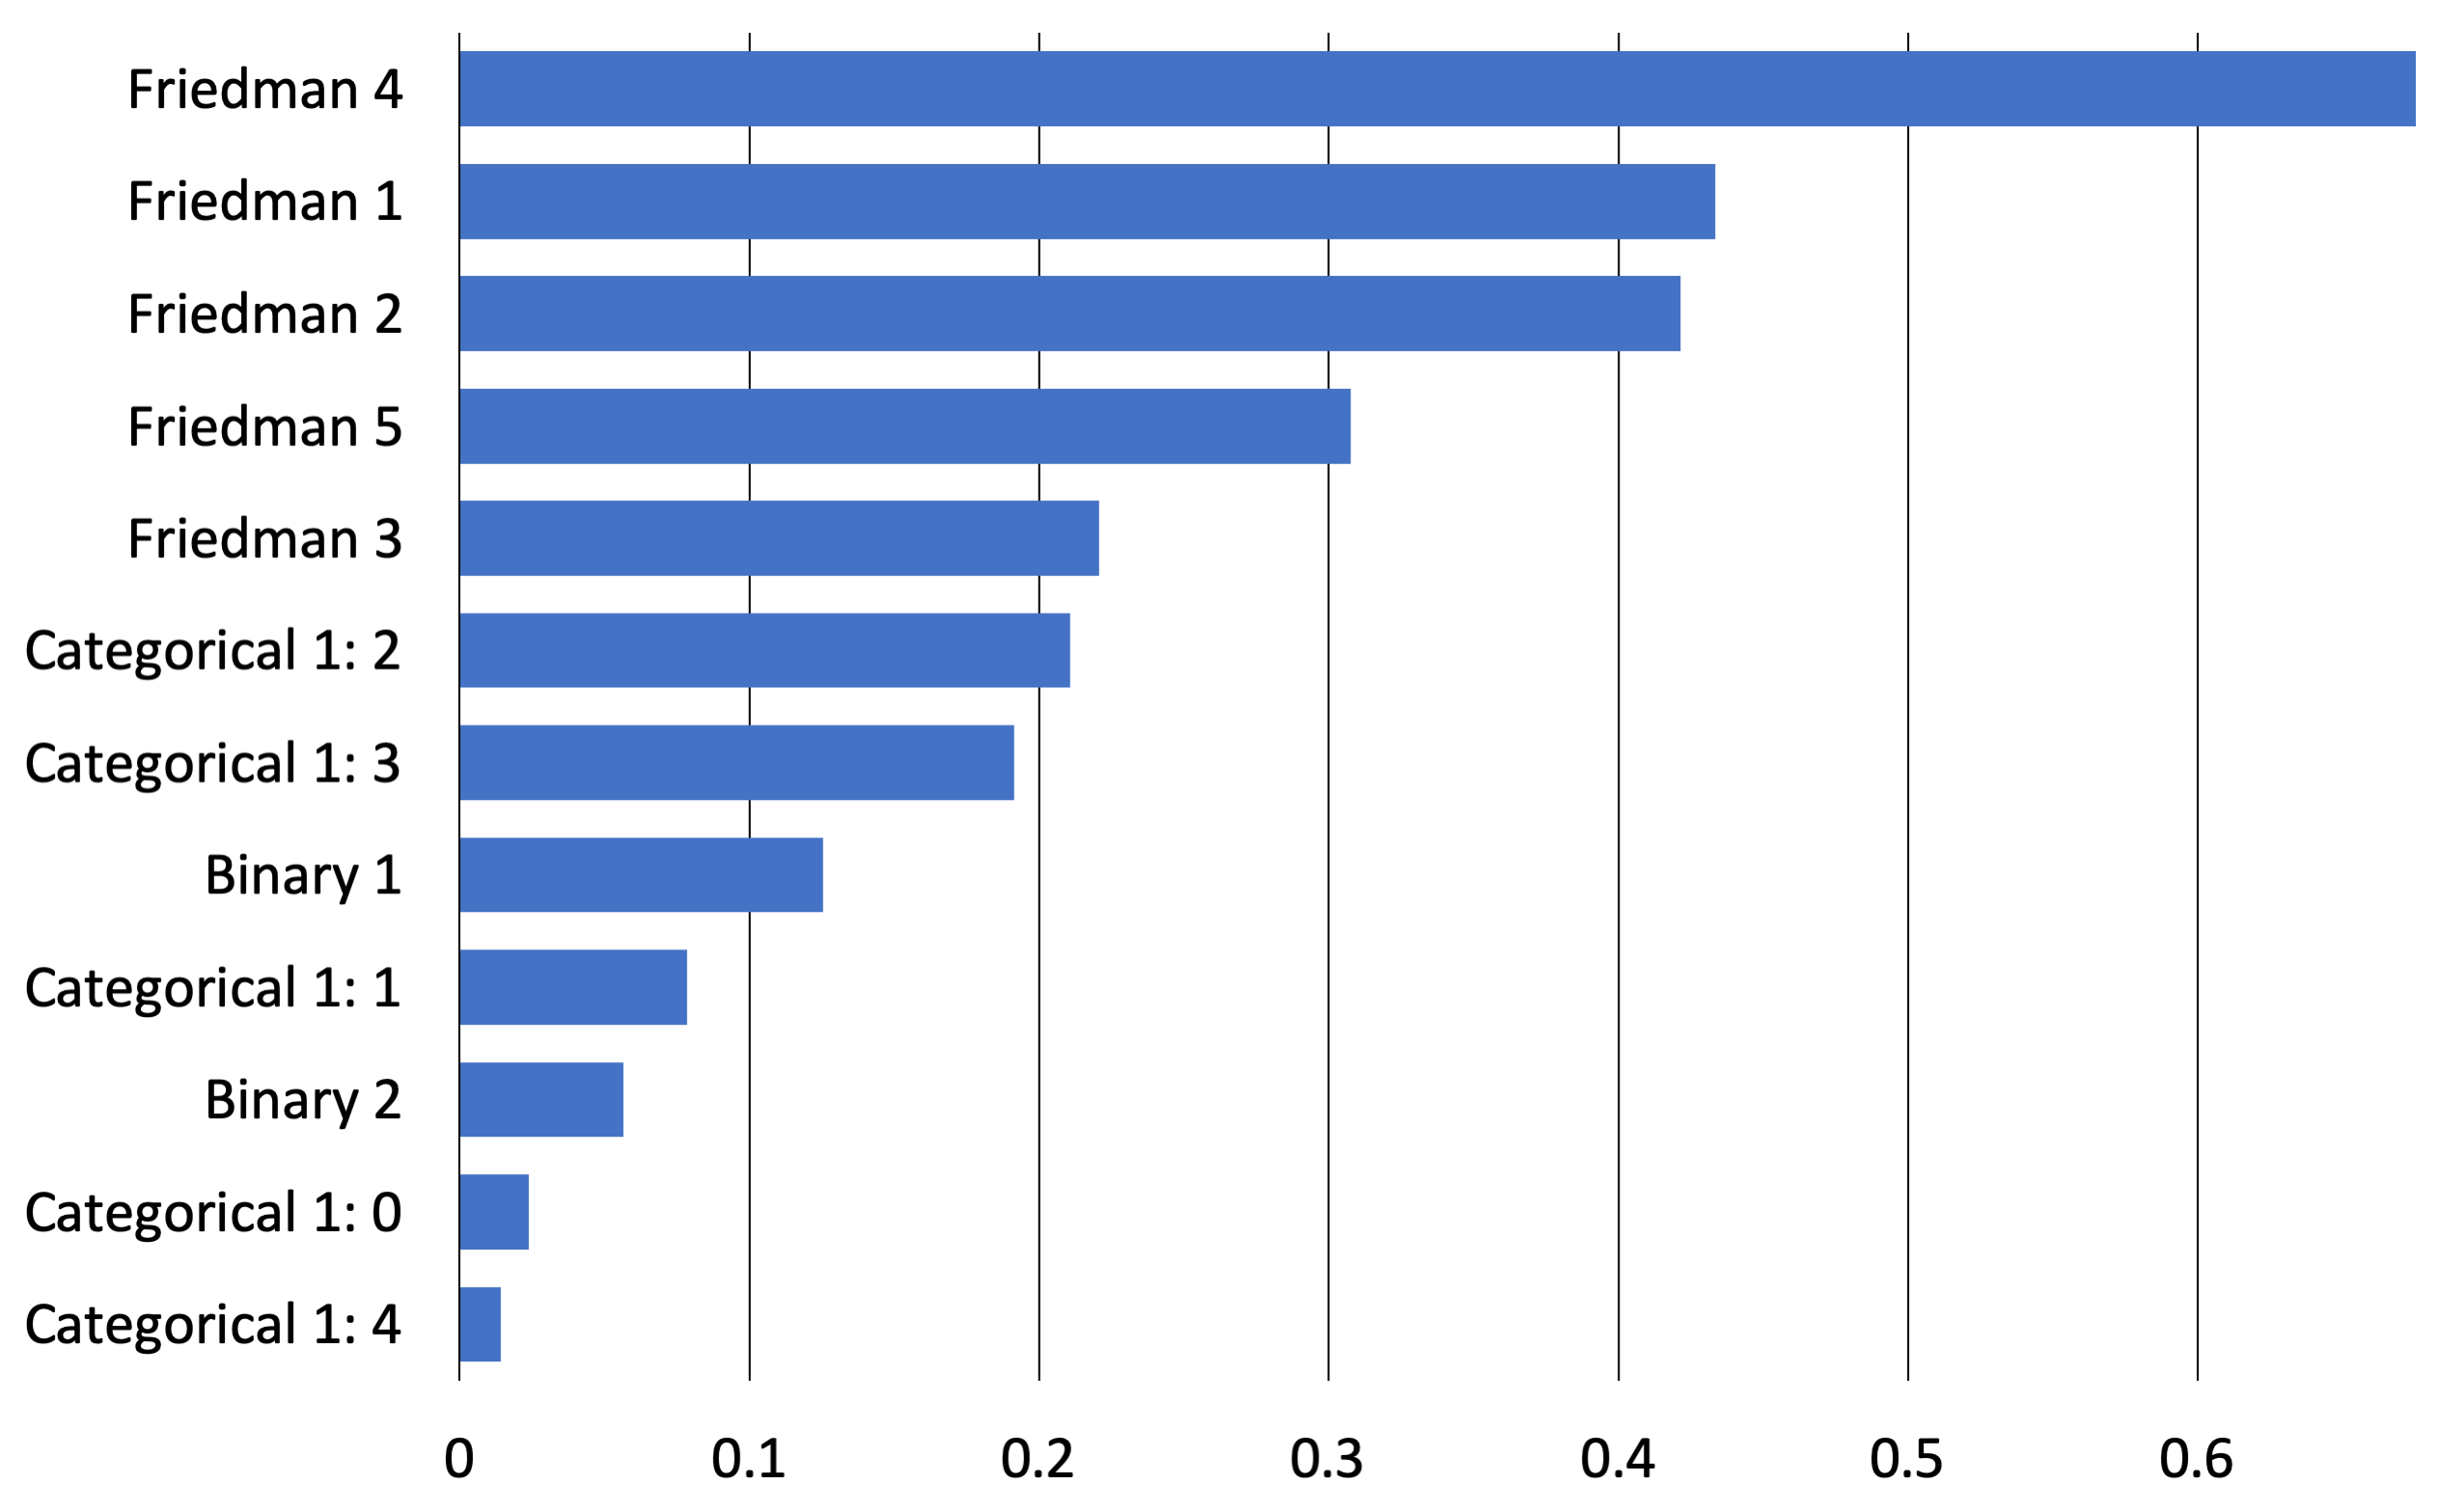
\includegraphics[width=8cm]{img/sim_mgbm_glob.png}
\label{fig:sim_mgbm_glob}
\caption{Global mean Tree SHAP feature importance for $g^\text{MGBM}$ on the simulated test data. Tree SHAP values are reported in the margin space, prior to the application of the logit link function.}
\end{figure}   

\begin{figure}[H]
\centering
\includegraphics[width=15cm]{img/sim_mgbm_glob_pdp_ice.png}
\label{fig:sim_mgbm_glob_pdp_ice}
\caption{PD, ICE for 10 observations across selected percentiles of $g^\text{MGBM}(\mathbf{X})$, and histograms for the three most important input features of $g^\text{MGBM}$ on the simulated test data.}
\end{figure}   

% highlight monotonicity 

\begin{figure}[H]
\centering
\includegraphics[width=15cm]{img/sim_mgbm_loc.png}
\label{fig:sim_mgbm_loc}
\caption{Tree SHAP values for three observations across selected percentiles of $g^\text{MGBM}(\mathbf{X})$ for the simulated test data. Tree SHAP values are reported in the margin space, prior to the application of the logit link function.}
\end{figure}   

\begin{figure}[H]
\centering
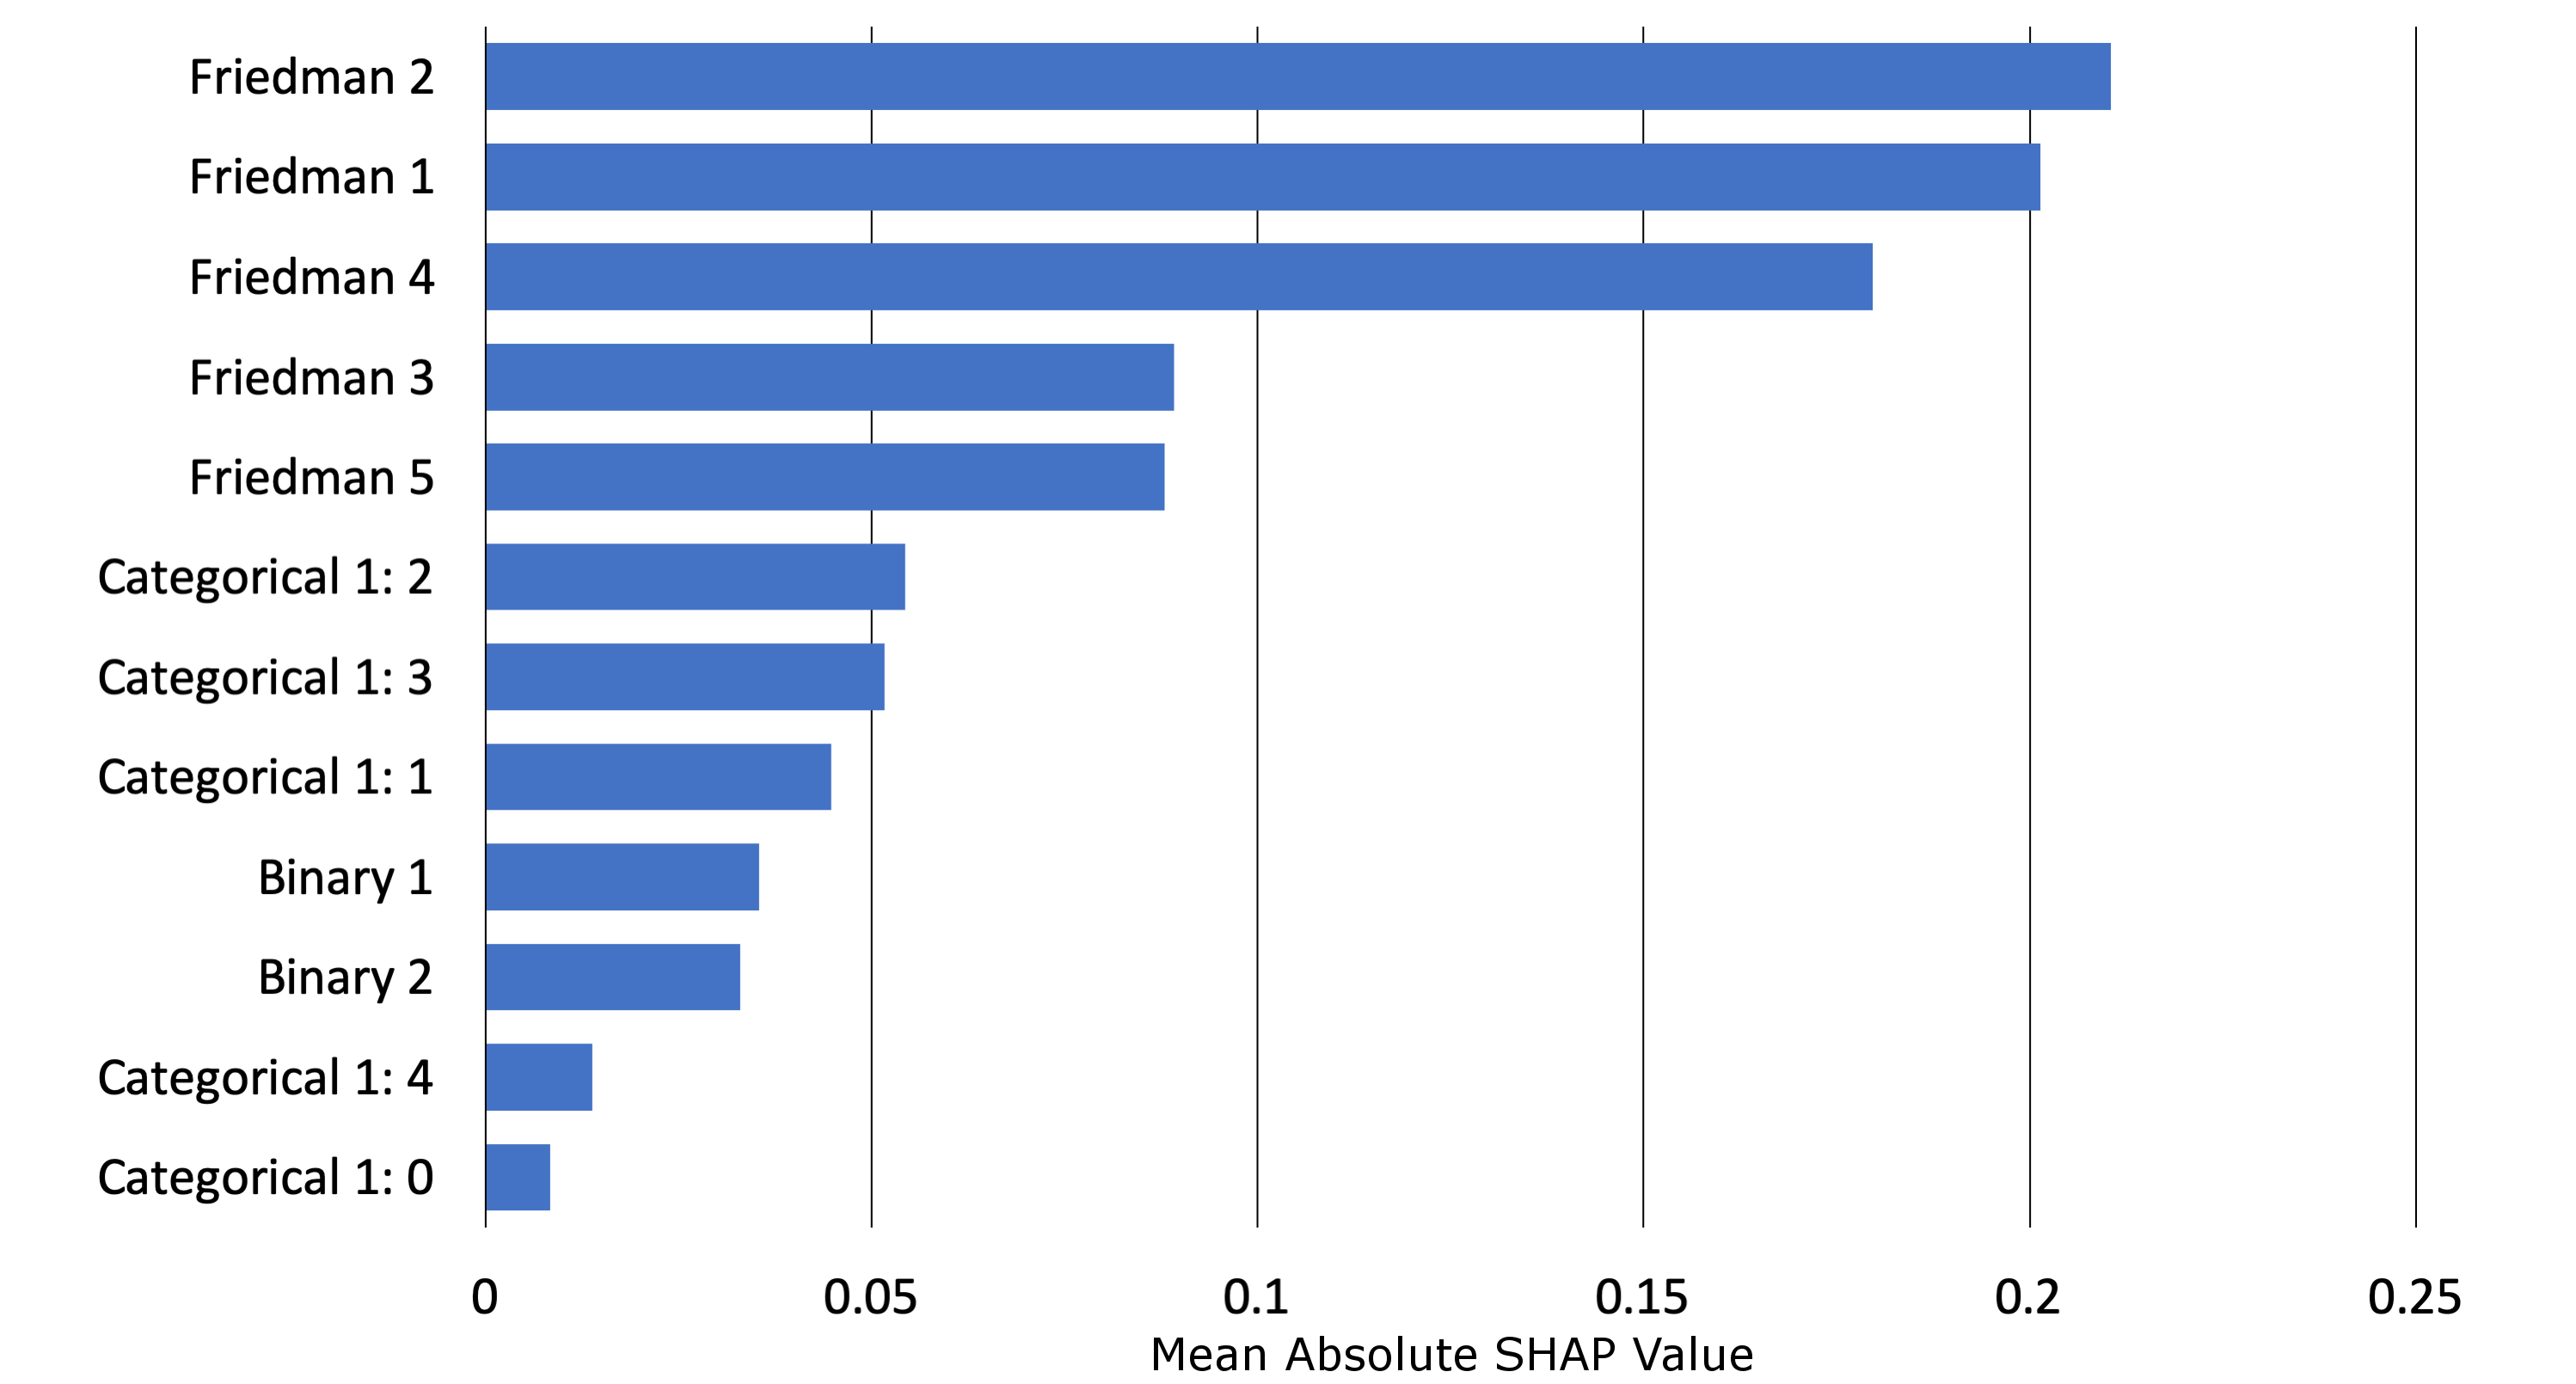
\includegraphics[width=8cm]{img/sim_xnn_glob.png}
\label{fig:sim_xnn_glob}
\caption{Global mean Deep SHAP feature importance for $g^\text{XNN}$ on the simulated test data.}
\end{figure} 

\begin{figure}[H]
\centering
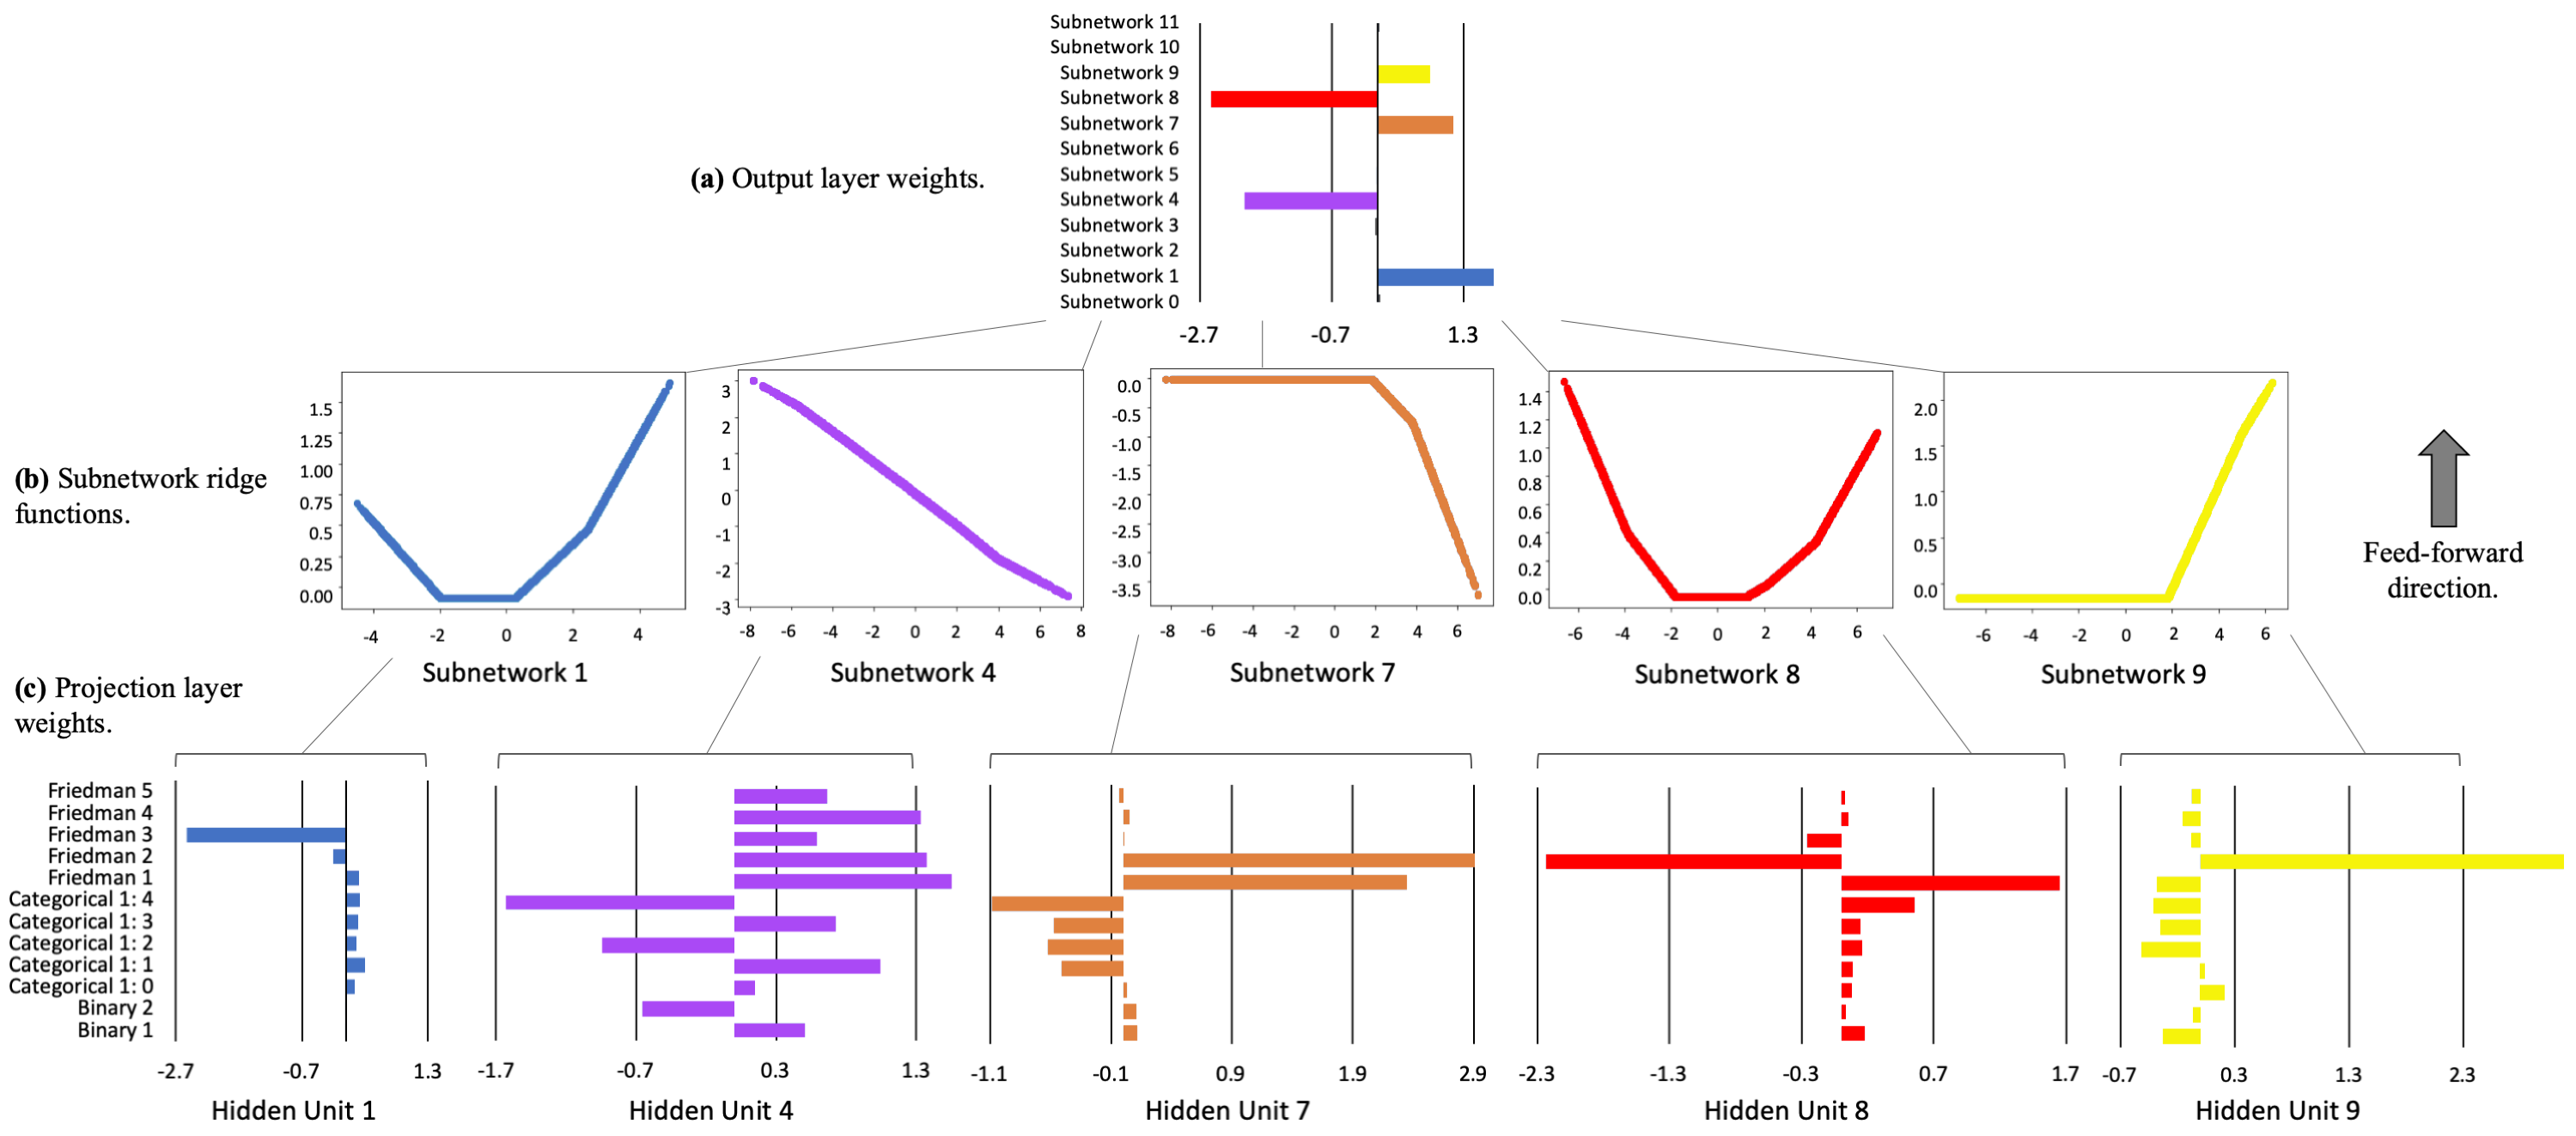
\includegraphics[width=17cm]{img/sim_xnn_glob_ridge.png}
\label{fig:sim_xnn_glob_ridge}
\caption{Ridge functions for the three most important input features for $g^\text{XNN}$ on the simulated test data.}
\end{figure}   

\begin{figure}[H]
\centering
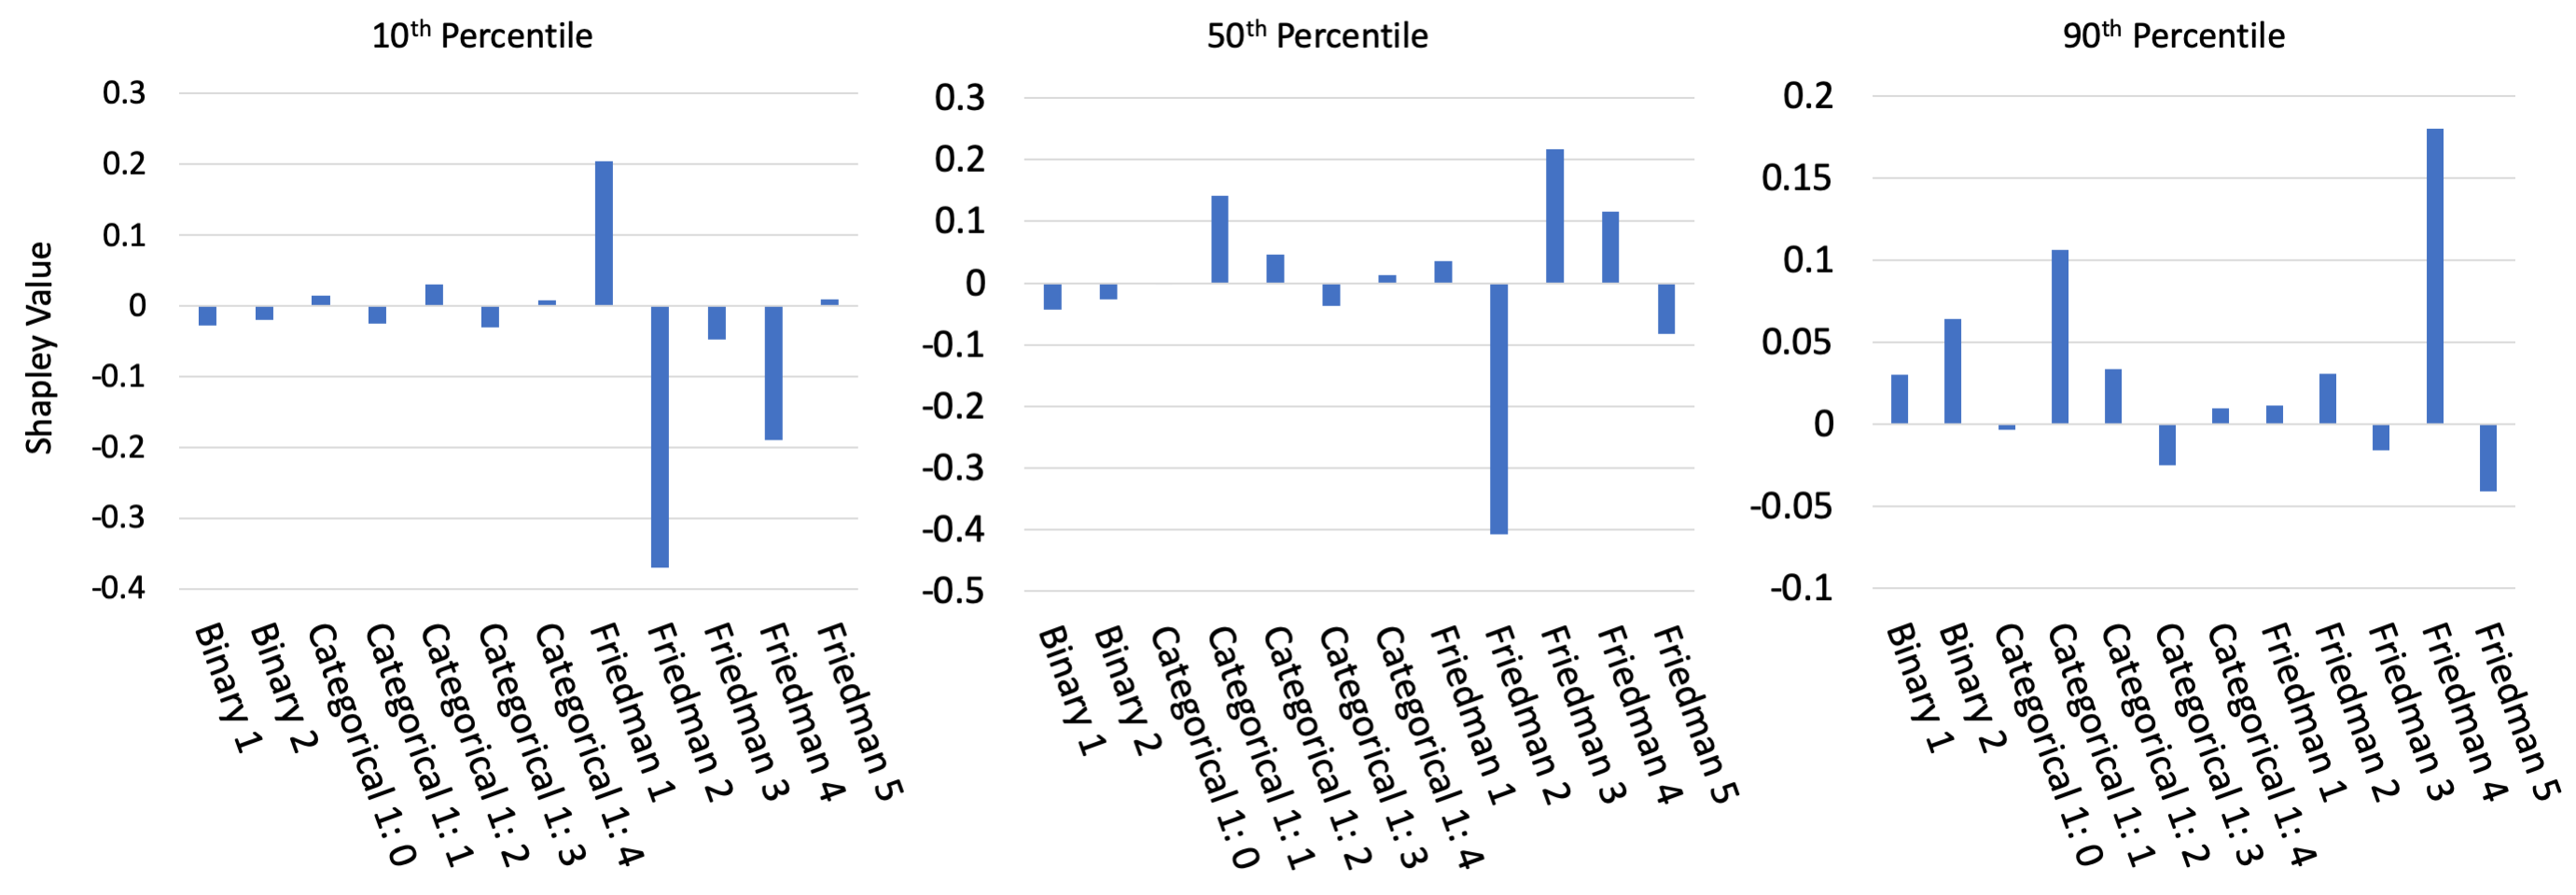
\includegraphics[width=15cm]{img/sim_xnn_loc.png}
\label{fig:sim_xnn_loc}
\caption{Deep SHAP values for three observations across selected percentiles of  $g^\text{XNN}$ on the simulated test data. Deep SHAP values are reported in the probability space, after the application of the logit link function.}
\end{figure}  

\subsubsection{Discrimination Testing Results}

%%%%%%%%%%%%%%%%%%%%%%%%%%%%%%%%%%%%%%%%%%
\subsection{Mortgage Data Results}

\subsubsection{Constrained vs. Unconstrained Model Fit Assessment}

\begin{table}[H]
\label{tab:mort_acc}
\caption{Fit metrics for $g^\text{GBM}$, $g^\text{MGBM}$, $g^\text{ANN}$, and $g^\text{XNN}$ on the mortgage test data. Accuracy is measured at the best F1 threshold for each model.}
\centering
%% \tablesize{} %% You can specify the fontsize here, e.g., \tablesize{\footnotesize}. If commented out \small will be used.
\begin{tabular}{ccccc}
\toprule
\textbf{Model}		& \textbf{Accuracy}	& \textbf{AUC}	 & \textbf{Logloss}	& \textbf{RMSE}\\
\midrule	
$g^\text{GBM}$		& 0.795	& 0.828	& 0.252	& 0.276 \\
$g^\text{MGBM}$	& 0.765	& 0.814	& 0.259	& 0.278 \\
$g^\text{ANN}$		& 0.860	& 0.872 	& 0.230 	& 0.262 \\
$g^\text{XNN}$		& 0.869	& 0.868	& 0.233	& 0.263 \\
\bottomrule
\end{tabular}
\end{table}

\subsubsection{Interpretability and Post-hoc Explanation Results}

\begin{figure}[H]
\centering
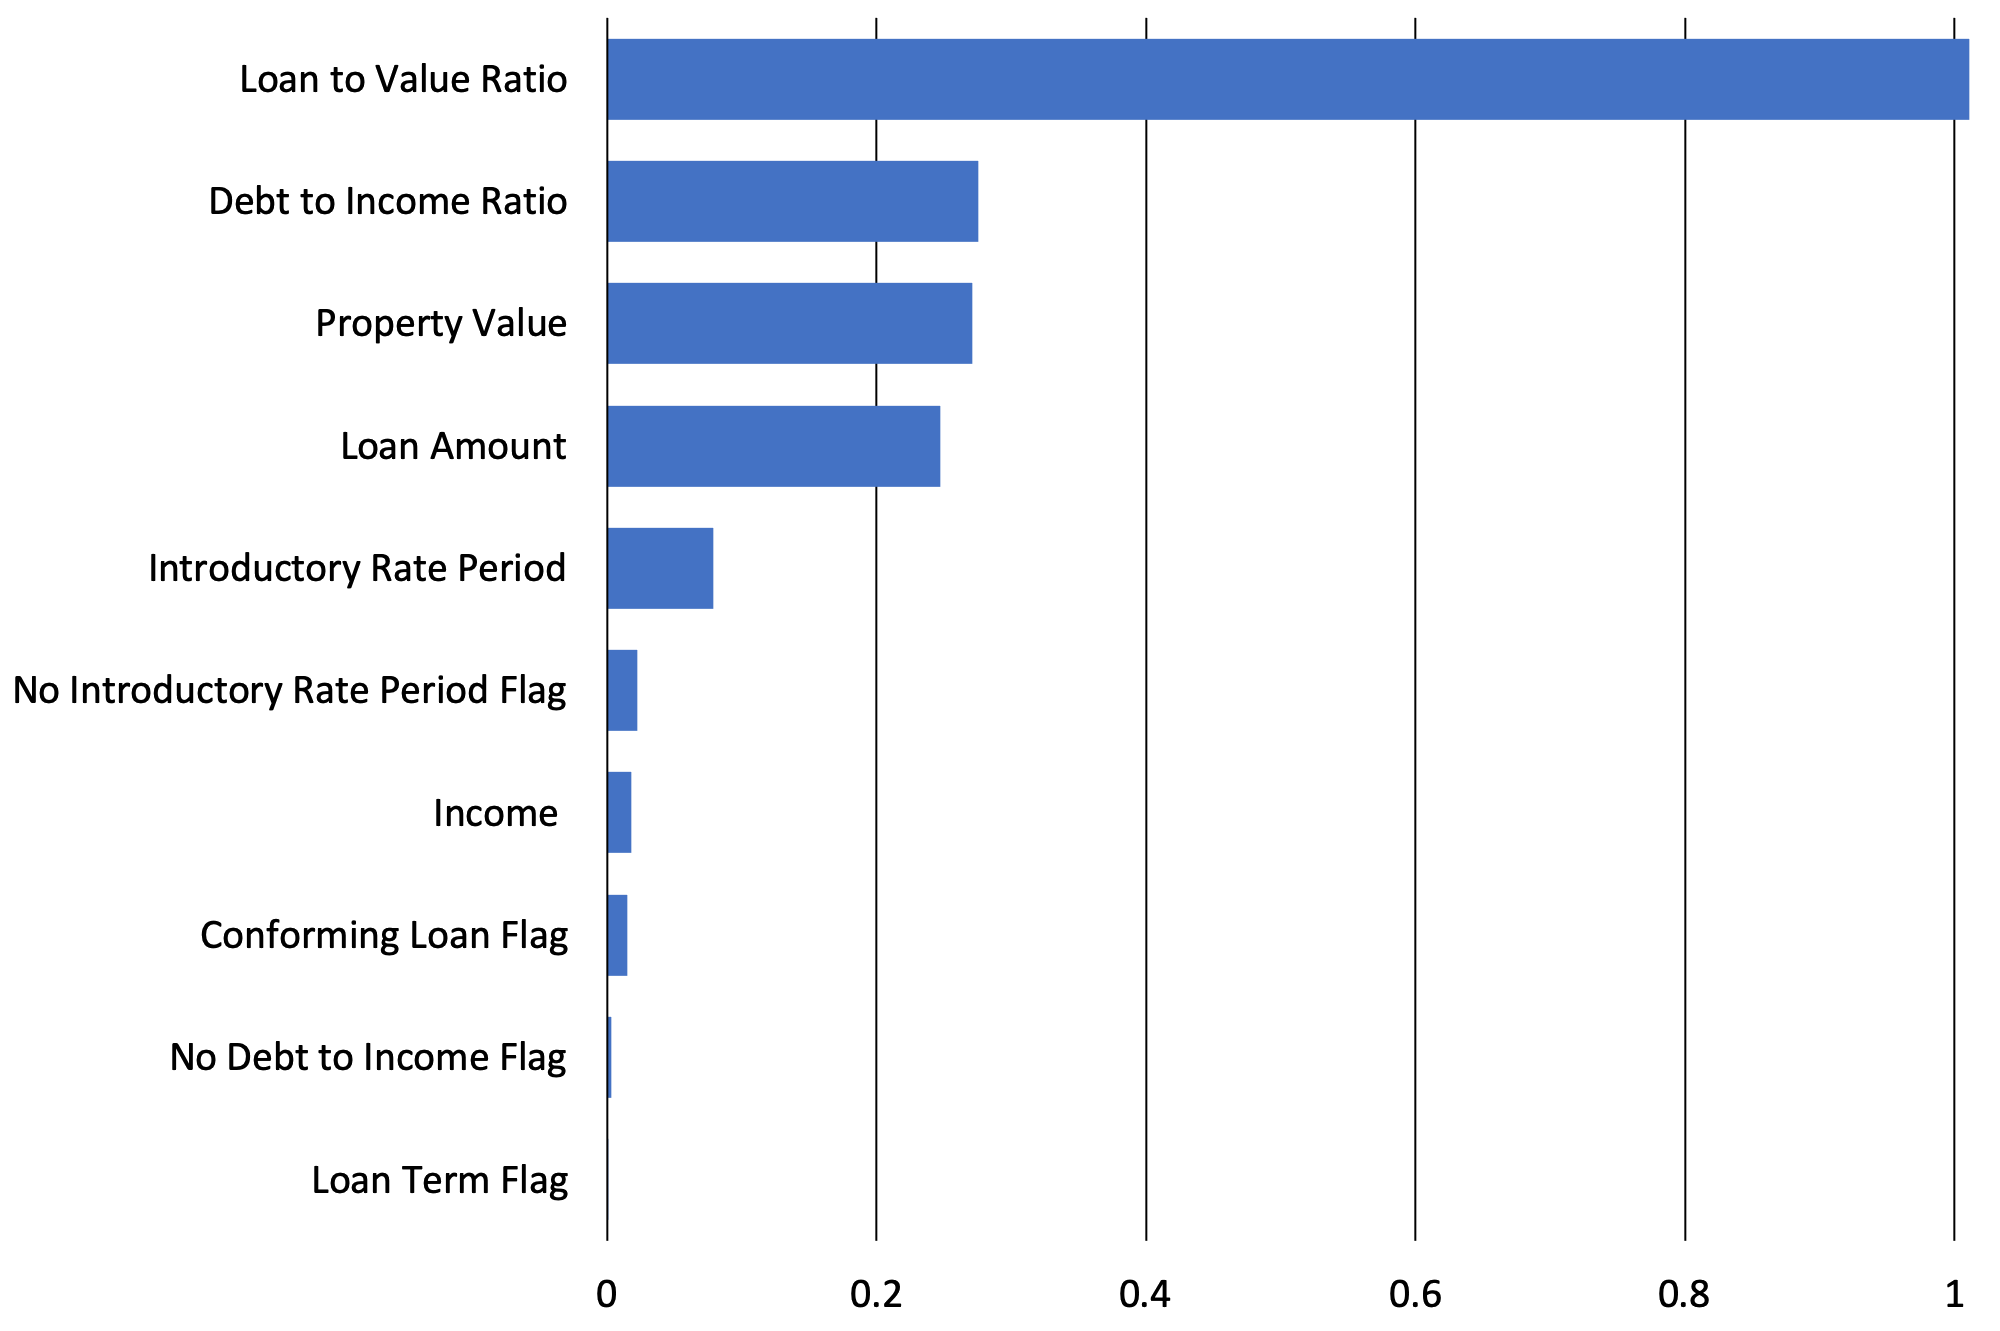
\includegraphics[width=8cm]{img/mort_mgbm_glob.png}
\label{fig:mort_mgbm_glob}
\caption{Global mean absolute Tree SHAP feature importance for $g^\text{MGBM}$ on the mortgage test data. Tree SHAP values are reported in the margin space, prior to the application of the logit link function.}
\end{figure} 

\begin{figure}[H]
\centering
\includegraphics[width=15cm]{img/mort_mgbm_glob_pdp_ice.png}
\label{fig:mort_mgbm_glob_pdp_ice}
\caption{PD, ICE for 10 individuals across selected percentiles of $g^\text{MGBM}(\mathbf{X})$, and histograms for the three most important input features of $g^\text{MGBM}$ on the mortgage test data.}
\end{figure}   

% highlight monotonicity 

\begin{figure}[H]
\centering
\includegraphics[width=15cm]{img/mort_mgbm_loc.png}
\label{fig:mort_mgbm_loc}
\caption{Tree SHAP values for three individuals across selected percentiles of $g^\text{MGBM}(\mathbf{X})$ for the mortgage test data. Tree SHAP values are reported in the margin space, prior to the application of the logit link function.}
\end{figure}   

\begin{figure}[H]
\centering
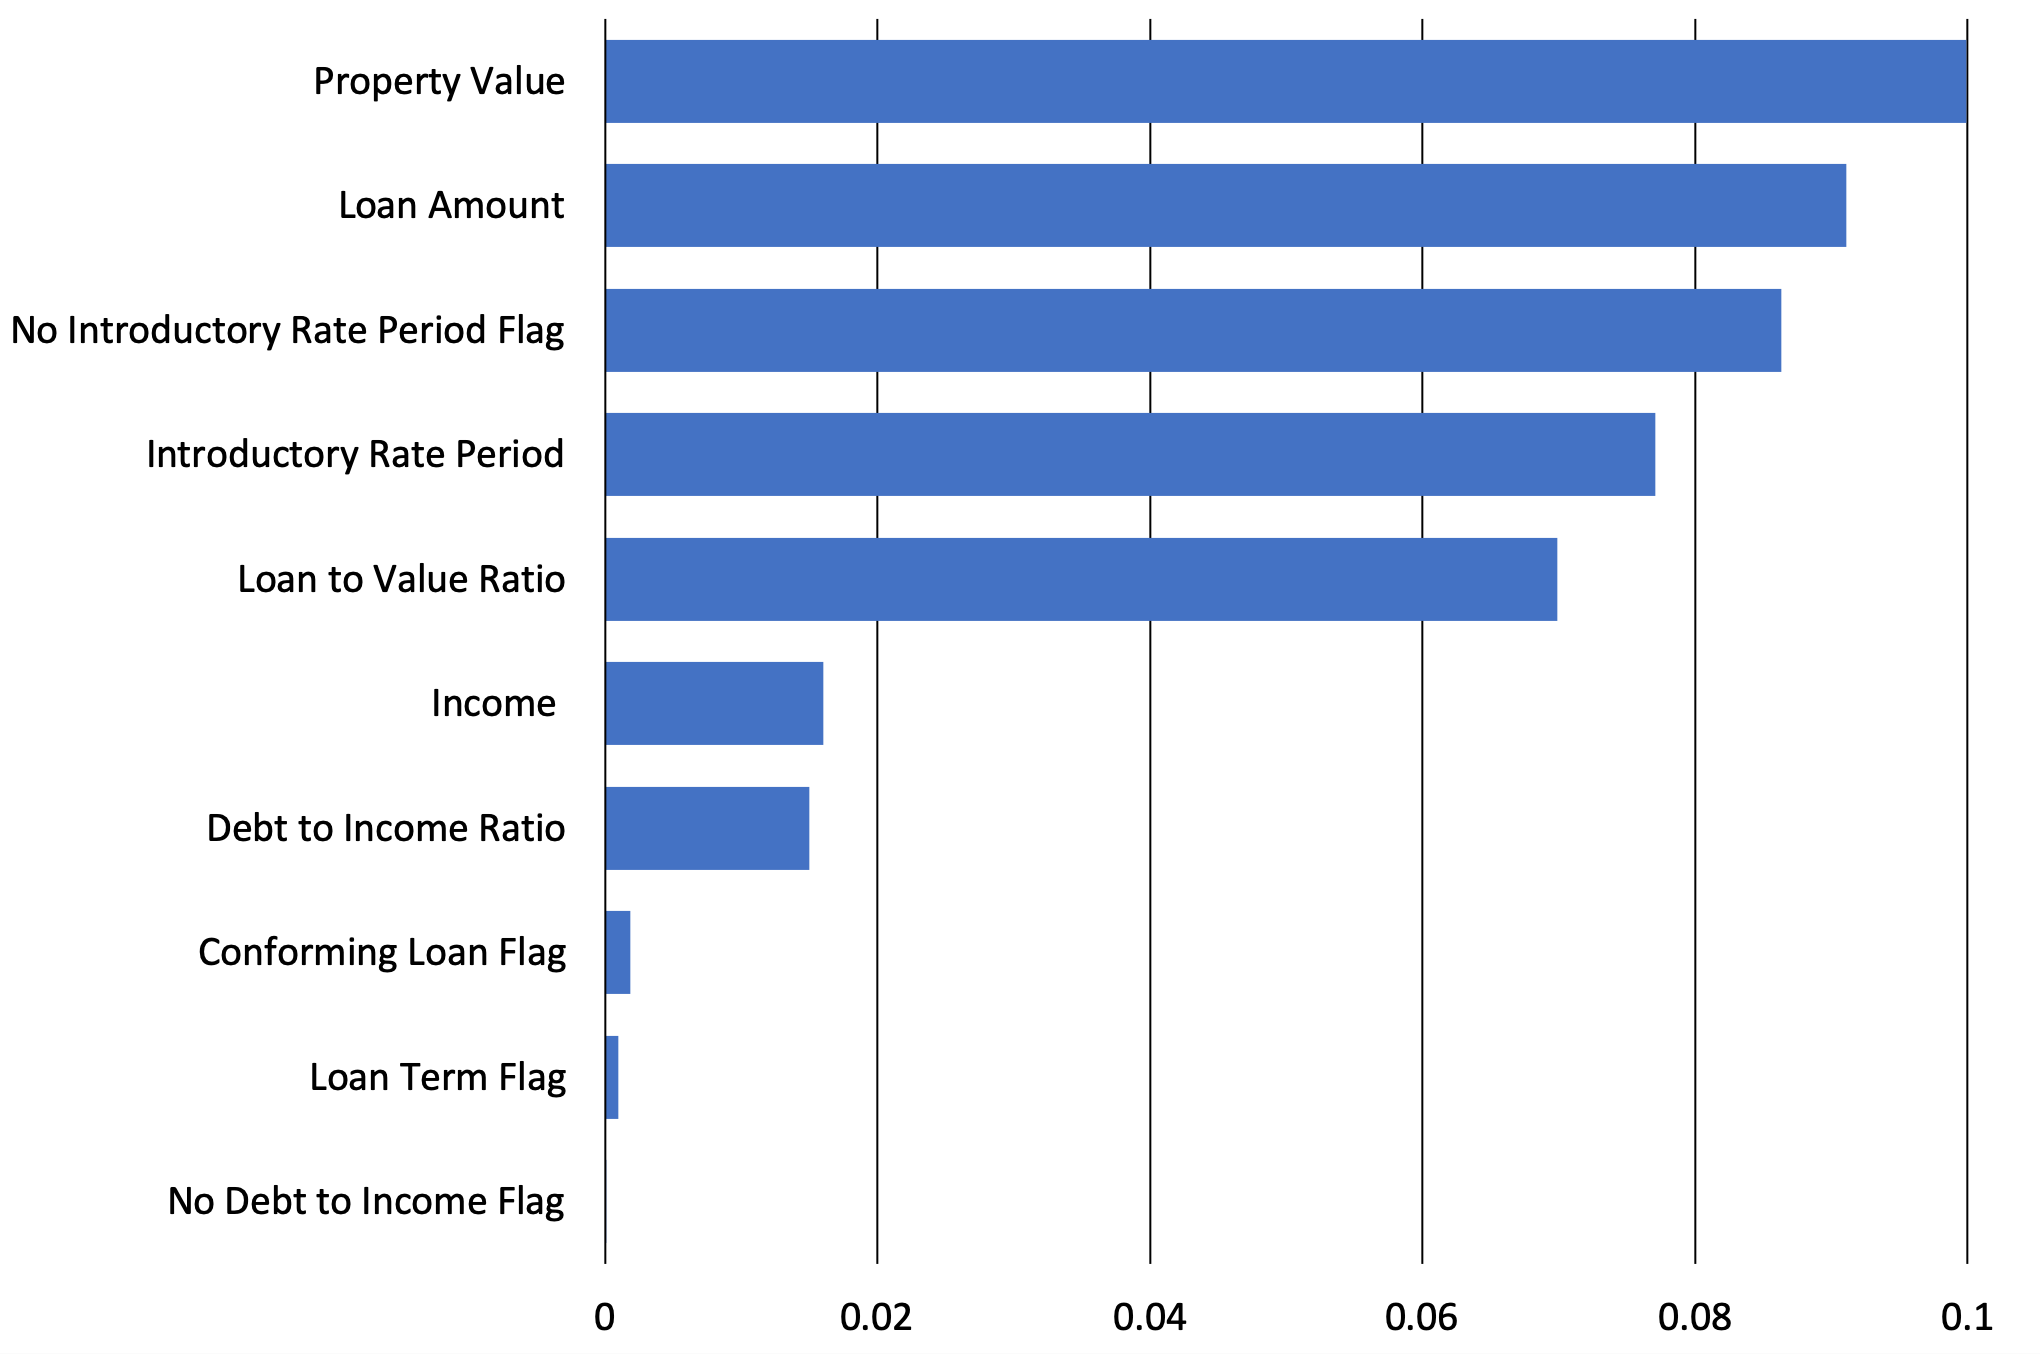
\includegraphics[width=8cm]{img/mort_xnn_glob.png}
\label{fig:mort_xnn_glob}
\caption{Global mean absolute Deep SHAP feature importance for $g^\text{XNN}$ on the mortgage test data. Deep SHAP values are reported in the probability space, after the application of the logit link function.}
\end{figure} 

\begin{figure}[H]
\centering
%\includegraphics[width=8cm]{img/}
\label{fig:mort_xnn_glob_pdp_ice}
\caption{Ridge functions for the three most important input features for $g^\text{XNN}$ on the mortgage test data. }
\end{figure}   

\begin{figure}[H]
\centering
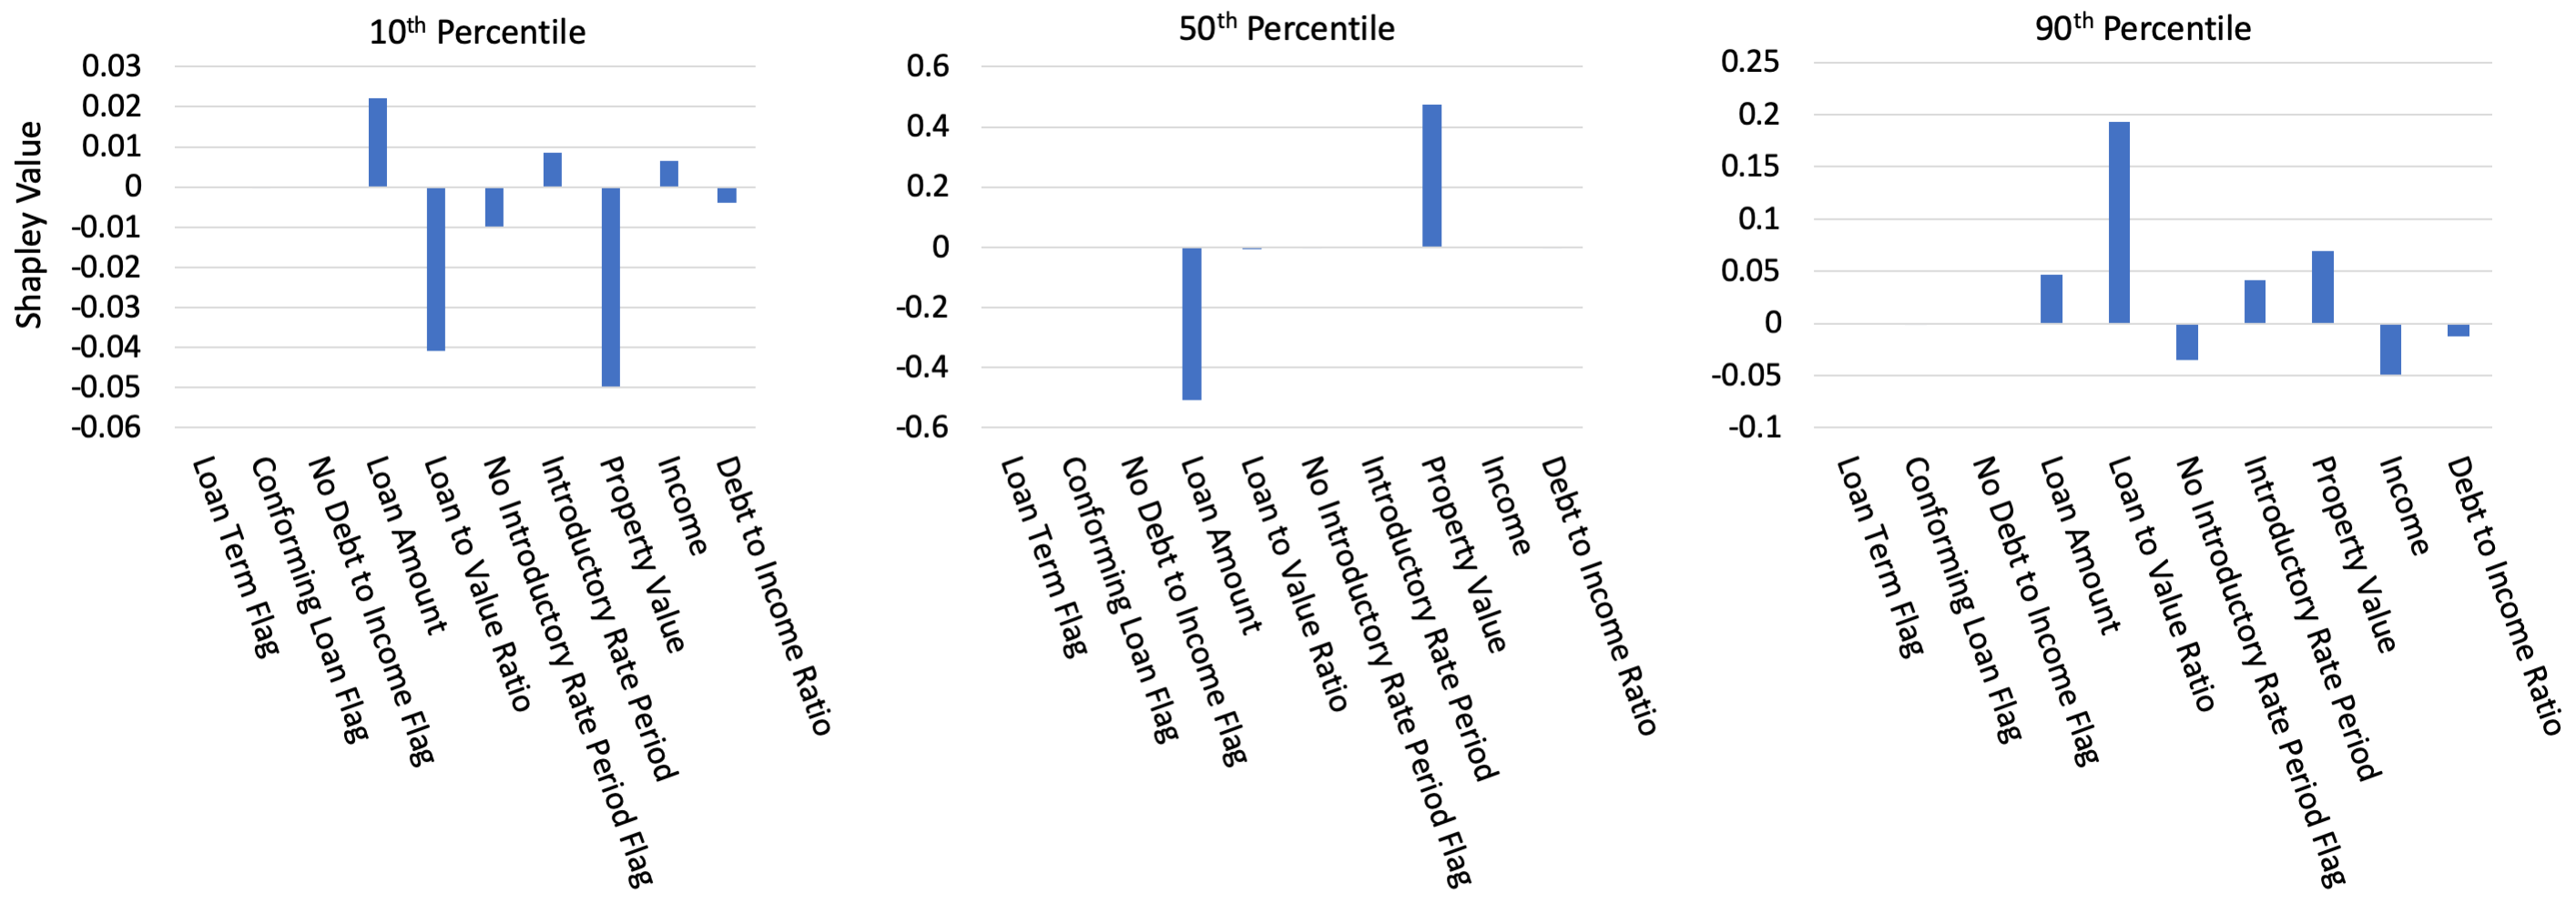
\includegraphics[width=15cm]{img/mort_xnn_loc.png}
\label{fig:mort_xnn_loc}
\caption{Deep SHAP values for three individuals across selected percentiles of $g^\text{XNN}$ on the mortgage test data. Deep SHAP values are reported in the probability space, after the application of the logit link function.}
\end{figure}

\subsubsection{Discrimination Testing Results}

%%%%%%%%%%%%%%%%%%%%%%%%%%%%%%%%%%%%%%%%%%
\section{Discussion}\label{sec:disc}

\subsection{The Burgeoning Python Ecosystem for Responsible Machine Learning}

MGBM and XNN interpretable model architectures were selected for this text because they are straightforward variants of popular unconstrained ML models. If practitioners are working with GBM and ANN models, it should be relatively uncomplicated for them to evaluate the constrained versions of these models. The same can be said of the presented explanation methods and discrimination tests. Due to their post-hoc nature, they can often be shoe-horned into existing ML work flows and pipelines. While these approaches are promising responses to the black-box and discrimination problems in ML, they are just a small part of a burgeoning ecosystem of research and Python tools for responsible ML. Figure \ref{fig:blueprint} is a work flow blueprint that illustrates some of the additional steps that may be required to build a fully understandable and trustworthy ML system.\footnote{See: \href{https://github.com/jphall663/hc_ml}{Toward Responsible Machine Learning} for details regarding Figure \ref{fig:blueprint}.} While all the methods mentioned in Figure \ref{fig:blueprint} play an important role in increasing human trust and understanding of ML, a few pertinent references and Python resources are highlighted below as further reading. 

\begin{figure}[H]
\centering
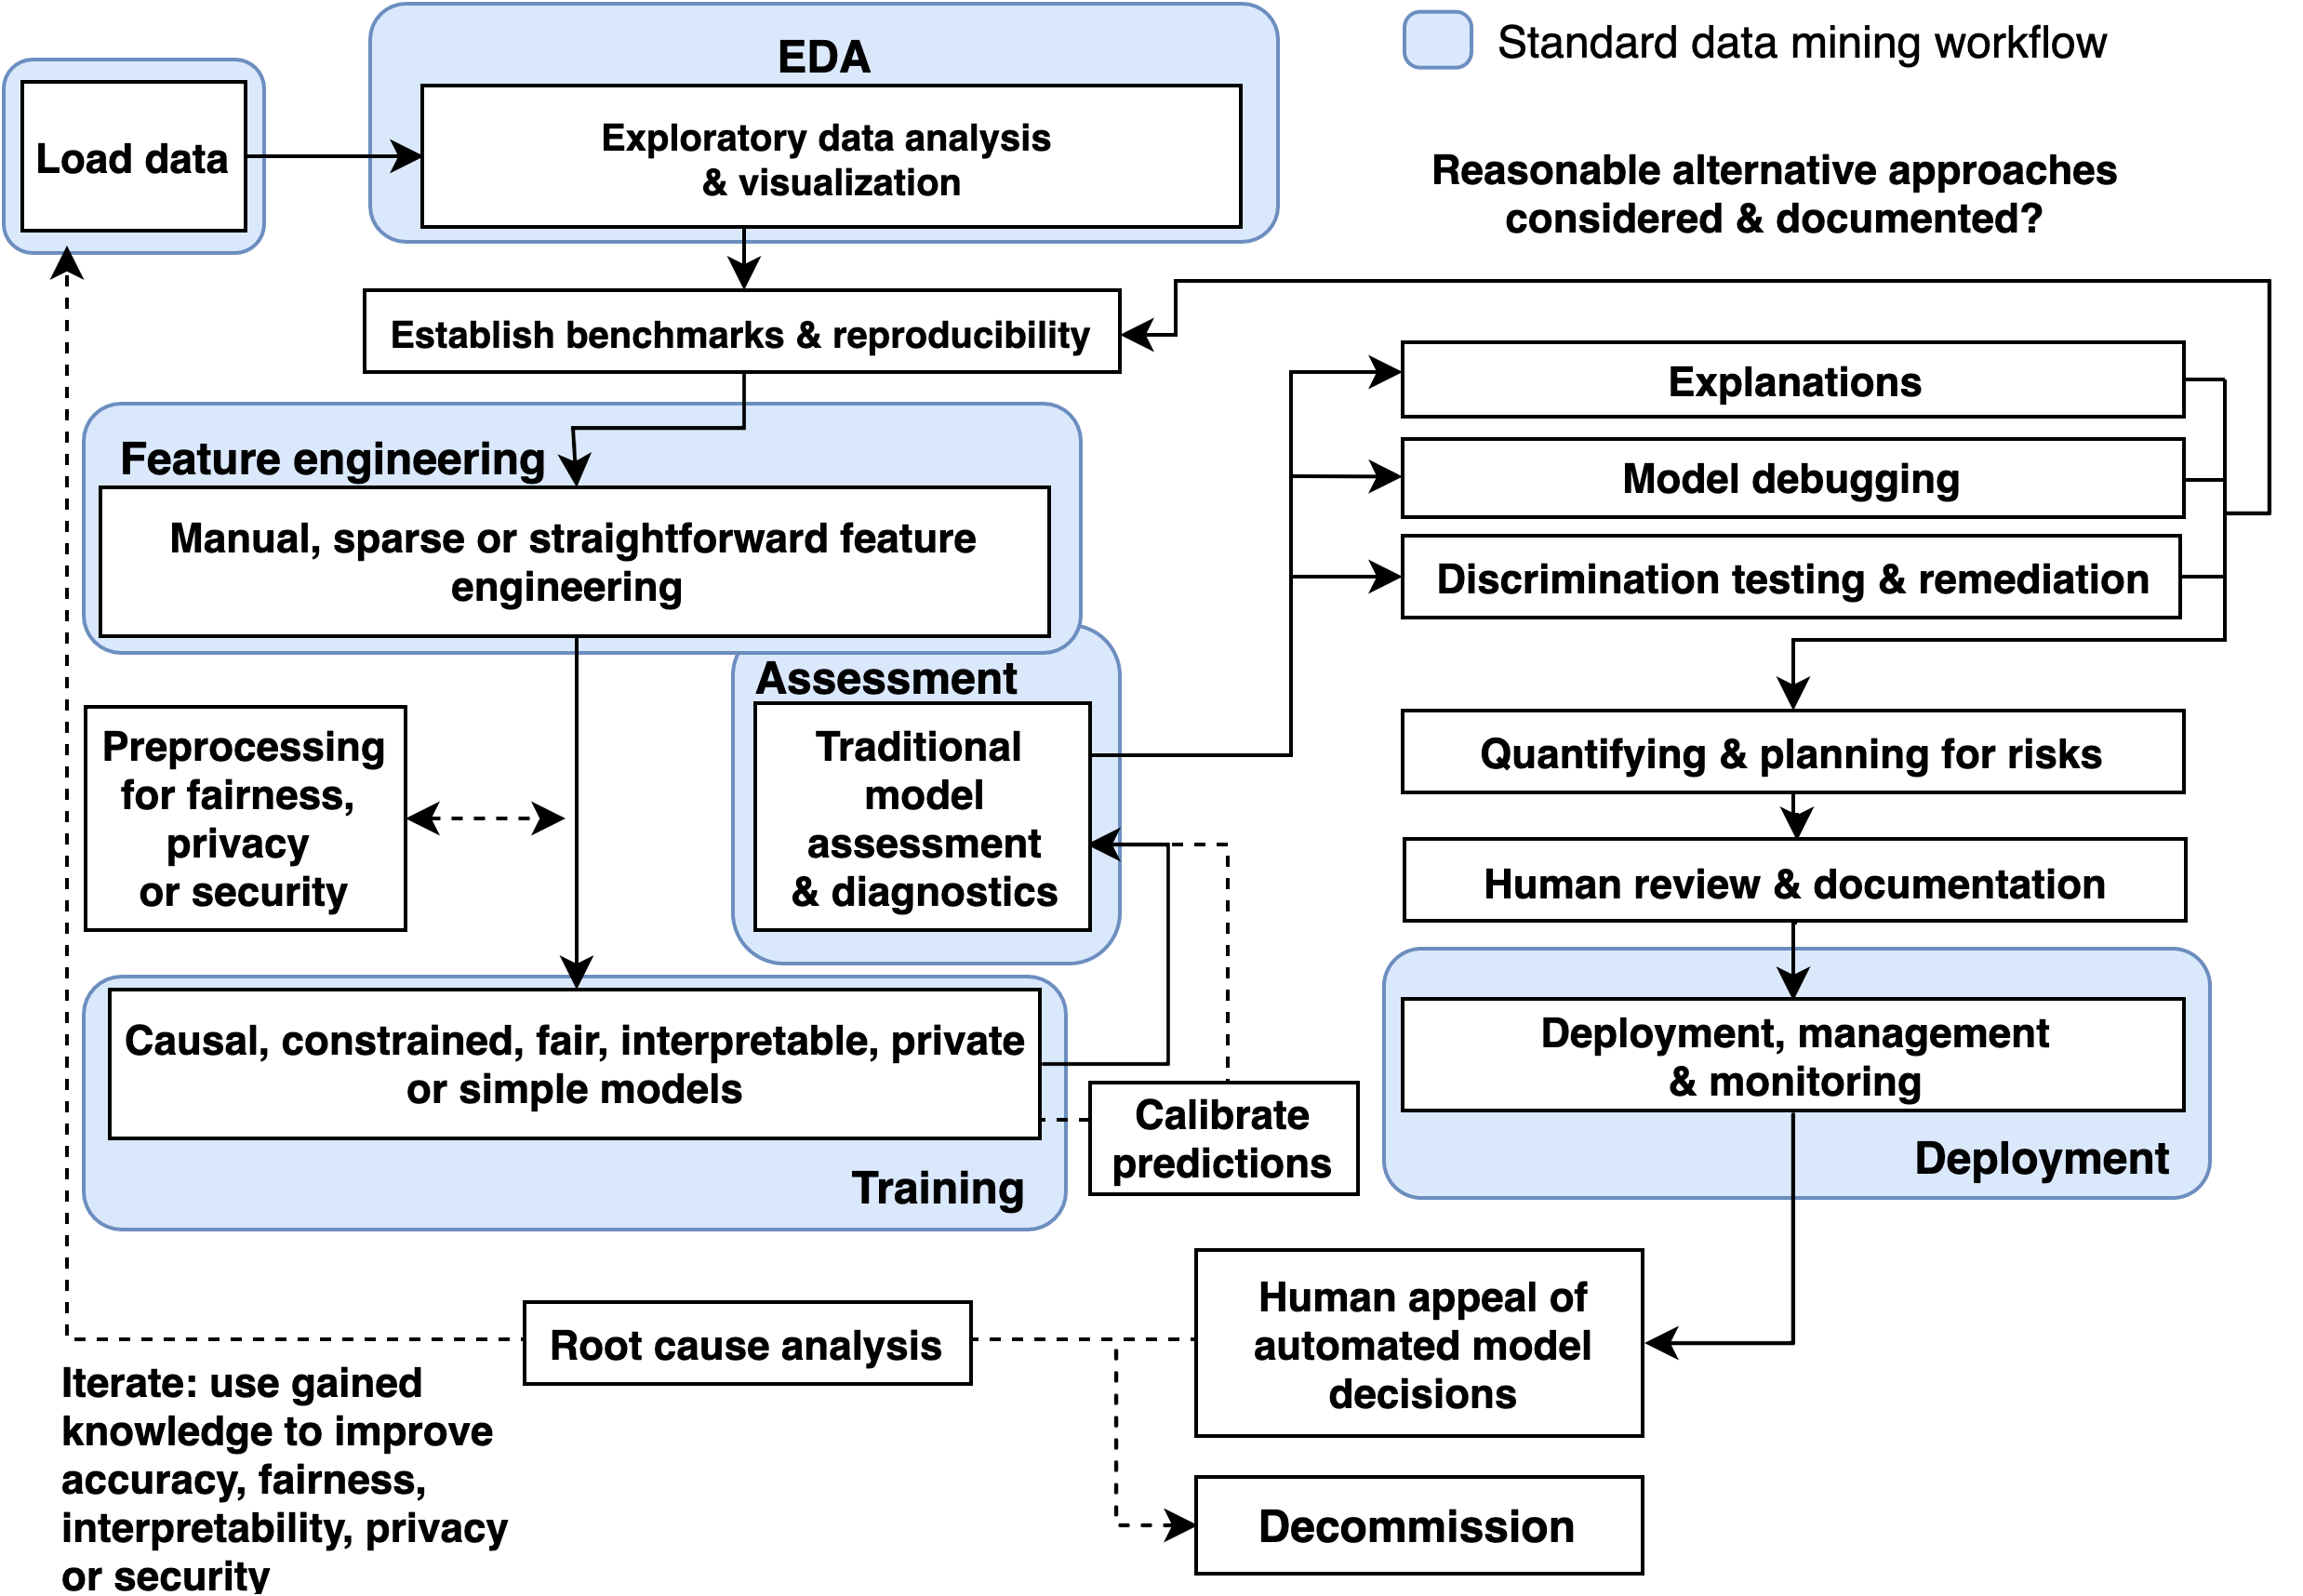
\includegraphics[width=8cm]{img/blueprint.png}
\caption{A diagram of a proposed holistic ML work flow in which interpretable models, post-hoc explanations, discrimination testing and remediation techniques, and other review and appeal mechanisms can create an understandable and trustworthy ML system.}
\label{fig:blueprint}
\end{figure}   

Any discussion of interpretable ML models would be incomplete without references to the seminal work of the Rudin group at Duke University and EBM or GA\textsuperscript{2}M models, pioneered by researchers at Microsoft and Cornell. In keeping with a major theme of this manuscript, models from these leading researchers and several other kinds of interpretable ML models are now available as open source Python packages. Among others, practitioners can now evaluate EBM in the \href{https://github.com/interpretml/interpret}{\texttt{interpret}} package, optimal sparse decision trees, GAMs in the \href{https://github.com/dswah/pyGAM}{\texttt{pyGAM}} package, a variant of Friedman's RuleFit  in the \href{https://github.com/scikit-learn-contrib/skope-rules}{\texttt{skope-rules}} package, monotonic calibrated interpolated lookup tables in \href{https://github.com/tensorflow/lattice}{\texttt{tensorflow/lattice}}, and \textit{this looks like that} interpretable deep learning \cite{osdt}, \cite{rulefit}, \cite{lattice}, \cite{this_looks_like_that}.\footnote{See: \href{https://github.com/xiyanghu/OSDT}{Optimal sparse decision trees}.}\textsuperscript{,}\footnote{See: \href{https://github.com/cfchen-duke/ProtoPNet}{\textit{This looks like that} interpretable deep learning}.} Additional, relevant references and Python functionality include:

\begin{itemize}[leftmargin=*,labelsep=5.8mm]

\item \textbf{Exploratory data analysis (EDA)}: \texttt{H2OAggregatorEstimator} in \href{http://docs.h2o.ai/h2o/latest-stable/h2o-py/docs/modeling.html#h2oaggregatorestimator}{\texttt{h2o}} \cite{wilkinson2018visualizing}.

\item \textbf{Sparse feature extraction}: \texttt{H2OGeneralizedLowRankEstimator} in \href{http://docs.h2o.ai/h2o/latest-stable/h2o-py/docs/modeling.html#h2ogeneralizedlowrankestimator}{\texttt{h2o}} \cite{udell2016generalized}.

\item \textbf{Privacy preprocessing and private models}: differential privacy and private models in \href{https://github.com/IBM/differential-privacy-library}{\texttt{diffprivlib}} and \href{https://github.com/tensorflow/privacy/}{\texttt{tensorflow/privacy}} \cite{diffprivlib}, \cite{ji2014differential}, \cite{pate}, \cite{abadi2016deep}.

\item \textbf{Post-hoc explanation}: structured data explanations with \href{https://github.com/SeldonIO/alibi}{\texttt{alibi}} and \href{https://github.com/SauceCat/PDPbox}{\texttt{PDPbox}}, image classification explanations with \href{https://github.com/marcoancona/DeepExplain}{\texttt{DeepExplain}}, and natural language explanations with \href{https://github.com/allenai/allennlp}{\texttt{allennlp}} \cite{wachter2017counterfactual}, \cite{grad_attr}, \cite{wallace2019allennlp}. 

\item \textbf{Discrimination testing}: with \href{https://github.com/dssg/aequitas}{\texttt{aequitas}} and \href{https://github.com/LASER-UMASS/Themis}{\texttt{Themis}}.

\item \textbf{Discrimination remediation}: Reweighing, adversarial de-biasing, learning fair representations, and reject option classification with \href{http://aif360.mybluemix.net/}{\texttt{AIF360}} \cite{kamiran2012data}, \cite{zhang2018mitigating}, \cite{lfr}, \cite{kamiran2012decision}.

\item \textbf{Model debugging}: with \href{https://github.com/bethgelab/foolbox}{\texttt{foolbox}}, \href{https://github.com/SALib/SALib}{\texttt{SALib}}, \href{https://github.com/tensorflow/cleverhans}{\texttt{tensorflow/cleverhans}}, and \href{https://github.com/tensorflow/model-analysis}{\texttt{tensorflow/model-analysis}} \cite{rauber2017foolbox}, \cite{papernot2018cleverhans}, \cite{modeltracker}, \cite{papernot2018marauder}.

\item \textbf{Model documentation}: models cards \cite{model_cards}, e.g.  \href{https://github.com/openai/gpt-2/blob/master/model_card.md}{GPT-2 model card}, \href{https://modelcards.withgoogle.com/object-detection}{Object Detection model card}. 

\end{itemize}

\noindent See: \href{https://github.com/jphall663/awesome-machine-learning-interpretability}{Awesome Machine Learning Interpretability} for a longer, community-curated metalist of related software packages and resources. 

\subsection{Interpretability, Explainability, Appeal, and Compliance}

Interpretable model architectures and post-hoc explanations play an important role in increasing transparency into model mechanisms and predictions. As seen in Sections \ref{sec:m_and_m} and \ref{sec:res}, interpretable models often enable users to enforce domain knowledge-based constraints on model behavior, to ensure that models obey reasonable expectations, and to gain data-derived insights into the modeled problem domain. Post-hoc explanations generally help describe and summarize mechanisms and decisions, potentially yielding an even clearer understanding of ML models. Together they can allow for human learning from ML, certain types of regulatory compliance, and crucially, human appeal or override of automated model decisions \cite{art_and_sci}. Interpretable models and post-hoc explanations are likely good candidates for ML uses cases under the FCRA, ECOA, GDPR and other regulations that may require explanations of model decisions, and they are already used in the financial services industry today for model validation and other purposes.\footnote{See: \href{https://ww2.amstat.org/meetings/jsm/2019/onlineprogram/AbstractDetails.cfm?abstractid=303053}{\textit{Deep Insights into Explainability and Interpretability of Machine Learning Algorithms and Applications to Risk Management}}.}\textsuperscript{,}\footnote{Unfortunately, many non-consistent explanation methods can result in drastically different global and local feature importance values across different models trained on the same data or even for refreshing a model with augmented training data \cite{molnar}. Consistency and accuracy guarantees are perhaps a factor in the growing momentum behind Shapley values as a candidate technique for generating consumer-specific adverse action notices for explaining and appealing automated ML-based decisions in highly-regulated settings such as credit lending \cite{bracke2019machine}.} Writ large, transparency in ML also facilitates additional responsible AI processes such as model debugging, model documentation, and logical appeal and override processes, some which may also be required by applicable regulations.\footnote{E.g.: \href{https://www.federalreserve.gov/supervisionreg/srletters/sr1107.htm}{US Federal Reserve Bank Supervision and Regulation (SR) Letter 11-7: Guidance on Model Risk Management}.} Among these, appeal may deserve the most attention. ML models are often wrong.\footnote{``All models are wrong, but some are useful.'' -- George Box, Statistician (1919 - 2013)} For high-stakes, human-centered, or regulated applications that are trusted with mission- or life-critical decisions, the ability to appeal or override inevitable wrong decisions is not only a possible prerequisite for regulatory compliance, but also an important failsafe procedure for those affected by ML decisions.  

\subsection{Impact of Discrimination Testing on Model Use and Adoption}

\subsection{Viable Discrimination Remediation Approaches}

\subsection{Intersectionality of Interpretability, Explainability, Discrimination, and Security in ML}

The black-box nature of ML, the perpetuation or exacerbation of discrimination by ML, or the security vulnerabilities inherent in ML are each serious and difficult problems on their own. However, evidence is mounting that these harms can also manifest as complex intersectional challenges, e.g. the \textit{fairwashing} or \textit{scaffolding} of biased models with ML explanations, the privacy harms of ML explanations, or the adversarial poisoning of ML models to become discriminatory \cite{shokri2019privacy}, \cite{fair_washing}, \cite{scaffolding}.\footnote{See: \href{https://www.theguardian.com/technology/2016/mar/24/tay-microsofts-ai-chatbot-gets-a-crash-course-in-racism-from-twitter}{\textit{Tay, Microsoft's AI chatbot, gets a crash course in racism from Twitter}}.}\textsuperscript{,}\footnote{While the focus of this paper is not ML security, proposed best-practices from that field do point to transparency of ML systems as a mitigating factor for some ML attacks and hacks \cite{papernot2018marauder}. High system complexity is sometimes considered a mitigating influence as well \cite{hoare19811980}. This is sometimes known as the \textit{transparency paradox} in data privacy and security, and it likely applies to ML security as well, especially in the context of interpretable ML models and post-hoc explanation.\textsuperscript{17}}\textsuperscript{,}\footnote{See: \href{https://hbr.org/2019/12/the-ai-transparency-paradox}{\textit{The AI Transparency Paradox}}.} Again, this text makes no claims that the opacity, discrimination, or security problems in ML have been solved, even treated as independent problems. Instead, this text aims to highlight these issues as both singular entities and non-static intersectional phenomena. Practitioners should of course consider the discussed interpretable modeling, post-hoc explanation, and discrimination testing approaches as at least partial remedies to the black-box and discrimination issues in ML. However, they should also consider that explanations can ease model stealing, data extraction, and membership inference attacks and that explanations can mask ML discrimination. Additionally, high-stakes, human-centered, or regulated ML systems should generally be built and tested with robustness to adversarial attacks as a primary design consideration, and specifically to prevent ML models from being poisoned or otherwise altered to become discriminatory. Accuracy, discrimination, and security characteristics of a system can change over time as well. Simply testing for these problems at training time, as presented in Sections \ref{sec:m_and_m} and \ref{sec:res}, is not adequate for high-stakes, human-centered, or regulated ML systems. Accuracy, discrimination, and security should be monitored in real-time and over time, as long as a model is deployed.

%%%%%%%%%%%%%%%%%%%%%%%%%%%%%%%%%%%%%%%%%%
\section{Conclusion}\label{sec:con}

This text puts forward results on simulated data to provide a rough validation of constrained ML models, post-hoc explanation techniques, and discrimination testing methods. These same modeling, explanation, and discrimination testing approaches are then applied to more realistic mortgage data to provide an example of a responsible ML work flow for high-stakes, human-centered, or regulated ML applications. The discussed methodologies are solid steps toward interpretability, explanation, and minimal discrimination for ML decisions, which should ultimately enable increased fairness and logical appeal processes for ML decision subjects. Of course there is more to the responsible practice of ML than interpretable models, post-hoc explanation, and discrimination testing, even from a technology perspective, and Section \ref{sec:disc} also points out numerous additional references and open source Python software assets that are available to researchers and practitioners today to increase human trust and understanding in ML systems. While the messy, complex, and human problems of racism, sexism, privacy violations, and cyber crime can probably not be solved by technology alone, this work (and many, many others) illustrate numerous ways for ML practitioners to become part of the solution to these problems, instead of perpetuating and exacerbating them. 

%%%%%%%%%%%%%%%%%%%%%%%%%%%%%%%%%%%%%%%%%%
\vspace{6pt} 

%%%%%%%%%%%%%%%%%%%%%%%%%%%%%%%%%%%%%%%%%%
\authorcontributions{NG, data cleaning, GBM and MGBM assessment and results; PH, primary author; KM, ANN and XNN implementation, assessment, and results; NS, secondary author, data simulation and collection, and discrimination testing.}%For research articles with several authors, a short paragraph specifying their individual contributions must be provided. The following statements should be used ``conceptualization, X.X. and Y.Y.; methodology, X.X.; software, X.X.; validation, X.X., Y.Y. and Z.Z.; formal analysis, X.X.; investigation, X.X.; resources, X.X.; data curation, X.X.; writing--original draft preparation, X.X.; writing--review and editing, X.X.; visualization, X.X.; supervision, X.X.; project administration, X.X.; funding acquisition, Y.Y.'', please turn to the  \href{http://img.mdpi.org/data/contributor-role-instruction.pdf}{CRediT taxonomy} for the term explanation. Authorship must be limited to those who have contributed substantially to the work reported.}

%%%%%%%%%%%%%%%%%%%%%%%%%%%%%%%%%%%%%%%%%%
\funding{This work received no external funding.}

%%%%%%%%%%%%%%%%%%%%%%%%%%%%%%%%%%%%%%%%%%
\acknowledgments{Wen Phan for work in formalizing notation. \textcolor{red}{BLDS editor} for editing. Andrew Burt for ideas around ML transparency, model debugging, and the transparency paradox.} 

%%%%%%%%%%%%%%%%%%%%%%%%%%%%%%%%%%%%%%%%%%
\conflictsofinterest{XNN was first made public by the corporate model validation team at Wells Fargo bank. Wells Fargo is a customer of, and investor in, H2O.ai and a customer of BLDS, LLC.} 

%%%%%%%%%%%%%%%%%%%%%%%%%%%%%%%%%%%%%%%%%%
%% optional
\abbreviations{The following abbreviations are used in this text: 
AI -- artificial intelligence, 
AIR - adverse impact ratio,
ALE - accumulated local effect,
ANN -- artificial neural network, 
DI -- disparate impact, 
EBM or GA\textsuperscript{2}M -- explainable boosting machine, i.e. variants GAMs that consider two-way interactions and may incorporate boosting into training, 
ECOA - Equal Credit Opportunity Act,
EDA -- exploratory data analysis,
EU -- European Union,
FCRA -- Fair Credit Reporting Act,
GAM -- generalized additive model, 
GBM -- gradient boosting machine, 
GDPR - General Data Protection Regulation,
HMDA -- Home Mortgage Disclosure Act
ICE -- individual conditional expectation, 
MGBM -- monotonic gradient boosting machine, 
ML -- machine learning, 
PD -- partial dependence, 
SGD -- stochastic gradient descent, 
SHAP -- Shapley additive explanation,
SMD - standardized mean difference,
SR -- supervision and regulation, 
US -- United States, 
XNN -- explainable neural network.}

%%%%%%%%%%%%%%%%%%%%%%%%%%%%%%%%%%%%%%%%%%
\reftitle{References}

%=====================================
% References, variant A: external bibliography
%=====================================
\externalbibliography{yes}
\bibliography{article-information-2019}

%%%%%%%%%%%%%%%%%%%%%%%%%%%%%%%%%%%%%%%%%%
\end{document}


%%%%%%%%%%%%%%%%%%%%%%%%%%%%%%%%%%%%%%%%%%

%%%%%%%%%%%%%%%%%%%%%%%%%%%%%%%%%%%%%%%%%%

%%%%%%%%%%%%%%%%%%%%%%%%%%%%%%%%%%%%%%%%%%


%This section may be divided by subheadings. It should provide a concise and precise description of the experimental results, their interpretation as well as the experimental conclusions that can be drawn.
%\begin{quote}
%This section may be divided by subheadings. It should provide a concise and precise description of the experimental results, their interpretation as well as the experimental conclusions that can be drawn.
%\end{quote}



%%%%%%%%%%%%%%%%%%%%%%%%%%%%%%%%%%%%%%%%%%
%\subsection{Subsection}
%\unskip
%\subsubsection{Subsubsection}

%Bulleted lists look like this:
%\begin{itemize}[leftmargin=*,labelsep=5.8mm]
%\item	First bullet
%\item	Second bullet
%\item	Third bullet
%\end{itemize}

%Numbered lists can be added as follows:
%\begin{enumerate}[leftmargin=*,labelsep=4.9mm]
%\item	First item 
%\item	Second item
%\item	Third item
%\end{enumerate}

%The text continues here.

%\subsection{Figures, Tables and Schemes}

%All figures and tables should be cited in the main text as Figure 1, Table 1, etc.

%\begin{figure}[H]
%\centering
%
\includegraphics[width=2 cm]{Definitions/logo-mdpi}
%\caption{This is a figure, Schemes follow the same formatting. If there are multiple panels, they should be listed as: (\textbf{a}) Description of what is contained in the first panel. (\textbf{b}) Description of what is contained in the second panel. Figures should be placed in the main text near to the first time they are cited. A caption on a single line should be centered.}
%\end{figure}   
 
%Text

%Text

%\begin{table}[H]
%\caption{This is a table caption. Tables should be placed in the main text near to the first time they are cited.}
%\centering
%% \tablesize{} %% You can specify the fontsize here, e.g., \tablesize{\footnotesize}. If commented out \small will be used.
%\begin{tabular}{ccc}
%\toprule
%\textbf{Title 1}	& \textbf{Title 2}	& \textbf{Title 3}\\
%\midrule
%entry 1		& data			& data\\
%entry 2		& data			& data\\
%\bottomrule
%\end{tabular}
%\end{table}

%Text

%Text

%\begin{listing}[H]
%\caption{Title of the listing}
%\rule{\textwidth}{1pt}
%\raggedright Text of the listing. In font size footnotesize, small, or normalsize. Preferred format: left aligned and single spaced. Preferred border format: top border line and bottom border line.
%\rule{\textwidth}{1pt}
%\end{listing}


%\subsection{Formatting of Mathematical Components}

%This is an example of an equation:

%\begin{equation}
%a + b = c
%\end{equation}
%% If the documentclass option "submit" is chosen, please insert a blank line before and after any math environment (equation and eqnarray environments). This ensures correct linenumbering. The blank line should be removed when the documentclass option is changed to "accept" because the text following an equation should not be a new paragraph. 

%Please punctuate equations as regular text. Theorem-type environments (including propositions, lemmas, corollaries etc.) can be formatted as follows:
%% Example of a theorem:
%\begin{Theorem}
%Example text of a theorem.
%\end{Theorem}

%The text continues here. Proofs must be formatted as follows:

%% Example of a proof:
%\begin{proof}[Proof of Theorem 1]
%Text of the proof. Note that the phrase `of Theorem 1' is optional if it is clear which theorem is being referred to.
%\end{proof}
%The text continues here.

%%%%%%%%%%%%%%%%%%%%%%%%%%%%%%%%%%%%%%%%%%
%\section{Discussion}

%Authors should discuss the results and how they can be interpreted in perspective of previous studies and of the working hypotheses. The findings and their implications should be discussed in the broadest context possible. Future research directions may also be highlighted.

%%%%%%%%%%%%%%%%%%%%%%%%%%%%%%%%%%%%%%%%%%
%\section{Materials and Methods}

%Materials and Methods should be described with sufficient details to allow others to replicate and build on published results. Please note that publication of your manuscript implicates that you must make all materials, data, computer code, and protocols associated with the publication available to readers. Please disclose at the submission stage any restrictions on the availability of materials or information. New methods and protocols should be described in detail while well-established methods can be briefly described and appropriately cited.

%Research manuscripts reporting large datasets that are deposited in a publicly available database should specify where the data have been deposited and provide the relevant accession numbers. If the accession numbers have not yet been obtained at the time of submission, please state that they will be provided during review. They must be provided prior to publication.

%Interventionary studies involving animals or humans, and other studies require ethical approval must list the authority that provided approval and the corresponding ethical approval code. 

%%%%%%%%%%%%%%%%%%%%%%%%%%%%%%%%%%%%%%%%%%
%\section{Conclusions}

%This section is not mandatory, but can be added to the manuscript if the discussion is unusually long or complex.

%%%%%%%%%%%%%%%%%%%%%%%%%%%%%%%%%%%%%%%%%%
%\section{Patents}
%This section is not mandatory, but may be added if there are patents resulting from the work reported in this manuscript.

%%%%%%%%%%%%%%%%%%%%%%%%%%%%%%%%%%%%%%%%%%
%% optional
%\supplementary{The following are available online at \linksupplementary{s1}, Figure S1: title, Table S1: title, Video S1: title.}

% Only for the journal Methods and Protocols:
% If you wish to submit a video article, please do so with any other supplementary material.
% \supplementary{The following are available at \linksupplementary{s1}, Figure S1: title, Table S1: title, Video S1: title. A supporting video article is available at doi: link.}


%\noindent 
%\begin{tabular}{@{}ll}
%MDPI & Multidisciplinary Digital Publishing Institute\\
%DOAJ & Directory of open access journals\\
%TLA & Three letter acronym\\
%LD & linear dichroism
%\end{tabular}}

%%%%%%%%%%%%%%%%%%%%%%%%%%%%%%%%%%%%%%%%%%
%% optional
%\appendixtitles{no} %Leave argument "no" if all appendix headings stay EMPTY (then no dot is printed after "Appendix A"). If the appendix sections contain a heading then change the argument to "yes".
%\appendix
%\section{}
%\unskip
%\subsection{}
%The appendix is an optional section that can contain details and data supplemental to the main text. For example, explanations of experimental details that would disrupt the flow of the main text, but nonetheless remain crucial to understanding and reproducing the research shown; figures of replicates for experiments of which representative data is shown in the main text can be added here if brief, or as Supplementary data. Mathematical proofs of results not central to the paper can be added as an appendix.

%\section{}
%All appendix sections must be cited in the main text. In the appendixes, Figures, Tables, etc. should be labeled starting with `A', e.g., Figure A1, Figure A2, etc. 

% Please provide either the correct journal abbreviation (e.g. according to the “List of Title Word Abbreviations” http://www.issn.org/services/online-services/access-to-the-ltwa/) or the full name of the journal.
% Citations an


%=====================================
% References, variant B: internal bibliography
%=====================================
%\begin{thebibliography}{999}
% Reference 1
%\bibitem[Author1(year)]{ref-journal}
%Author1, T. The title of the cited article. {\em Journal Abbreviation} {\bf 2008}, {\em 10}, 142--149.
% Reference 2
%\bibitem[Author2(year)]{ref-book}
%Author2, L. The title of the cited contribution. In {\em The Book Title}; Editor1, F., Editor2, A., Eds.; %Publishing House: City, Country, 2007; pp. 32--58.
%\end{thebibliography}

% The following MDPI journals use author-date citation: Arts, Econometrics, Economies, Genealogy, Humanities, IJFS, JRFM, Laws, Religions, Risks, Social Sciences. For those journals, please follow the formatting guidelines on http://www.mdpi.com/authors/references
% To cite two works by the same author: \citeauthor{ref-journal-1a} (\citeyear{ref-journal-1a}, \citeyear{ref-journal-1b}). This produces: Whittaker (1967, 1975)
% To cite two works by the same author with specific pages: \citeauthor{ref-journal-3a} (\citeyear{ref-journal-3a}, p. 328; \citeyear{ref-journal-3b}, p.475). This produces: Wong (1999, p. 328; 2000, p. 475)


%%%%%%%%%%%%%%%%%%%%%%%%%%%%%%%%%%%%%%%%%%
%% optional
%\sampleavailability{Samples of the compounds ...... are available from the authors.}

%% for journal Sci
%\reviewreports{\\
%Reviewer 1 comments and authors’ response\\
%Reviewer 2 comments and authors’ response\\
%Reviewer 3 comments and authors’ response
%}


